\documentclass{osa-article}

%% Select the journal you're submitting to
%% oe, boe, ome, osac, osajournal
\journal{oe}
% Key:
% Express journals must have the correct journal selected:
% {oe} Optics Express
% {boe} Biomedical Optics Express
% {ome} Optical Material Express
% {optcon} Optics Continuum
% Other OSA journals may use:
% {osajournal} Applied Optics, Advances in Optics and Photonics, Journal of the Optical Society of America A/B, Optics Letters, Optica, Photonics Research

% Uncomment if submitting to Photonics Research.
% ONLY APPLICABLE FOR \journal{osajournal}
% \setprjcopyright

% Set the article type
%\articletype{Research Article}
% Note that article type is not required for Express journals (OE, BOE, OME and OSAC)
% \usepackage[hang,small,bf]{caption}
\usepackage[subrefformat=parens]{subcaption}
\captionsetup{compatibility=false}
\usepackage{todonotes}
\usepackage{lineno}
\usepackage{layout}
\usepackage{lipsum}
\usepackage{bm, amsmath, comment, color, soul, cite, siunitx, physics}
\usepackage[capitalize]{cleveref}
\usepackage[super]{nth}
\sisetup{parse-numbers = false}
\linenumbers

\begin{document}

\title{Singlemode 1112\,nm and few-mode 976\,nm Yb-doped fiber amplifiers}

\author{Yasutaka IMAI\authormark{1, *}, Hideaki HARA\authormark{1}, Satoshi UETAKE\authormark{1}}

\address{\authormark{1}Reserch Institute for Interdisciplinary Science, Okayama University, Okayama, Japan}

\email{\authormark{*}imai1117@okayama-u.ac.jp} %% email address is required

% \homepage{http:...} %% author's URL, if desired

%%%%%%%%%%%%%%%%%%% abstract %%%%%%%%%%%%%%%%
%% [use \begin{abstract*}...\end{abstract*} if exempt from copyright]
\begin{comment}
  The abstract should be limited to approximately 100 words
  If the work of another author is cited in the abstract, that citation should be written out without a number, (e.g., journal, volume, first page, and year in square brackets [Opt. Express {\bfseries 22}, 1234 (2014)]), and a separate citation should be included in the body of the text
  The first reference cited in the main text must be [1]
  Do not include numbers, bullets, or lists inside the abstract.
\end{comment}
\begin{abstract}
We reported on a single stage \SI{976}{nm} Yb-doped fiber amplifier(YDFA) and a double stage \SI{1112}{nm} YDFA with commercially available Yb-doped fibers.
In developing of two YDFAs of different wavelengths, we estimated upper limit of Yb-doped fiber length and output of signal and ASE by numerical simulation.
The simulation results showed good agreement with experimental results, and both YDFAs achieved stable several Watts continuous-wave(CW) outputs\todo{need to be rewritten depending on simulation result}.
\end{abstract}

%%%%%%%%%%%%%%%%%%%%%%%%%%  body  %%%%%%%%%%%%%%%%%%%%%%%%%%
\listoftodos
\section{Introduction}
Rare-earth-doped fiber laser and amplifier systems are useful in a various fields.
For example, the high-power and compact systems are used in laser processing, long-distance optical communication, and LiDAR systems.
In physics, highly stable doped fiber systems are attractive as a light source for experiment \cite{burkley2017yb, coluccelli2016optical}.
Although there are still some problems which are not fully understood such as photodarkening \cite{paschotta1997lifetime}, remarkable progress has been made in their performance.

Single-frequency light sources at \SI{976}{nm} and \SI{1112}{nm} also such as spectroscopy of Yb atoms \todo{incomplete sentence} \cite{franzen2018singlestage}.
However, they are difficult to design because \SI{976}{nm} is in the middle of the absorption band and \SI{1112}{nm} is at the edge of the emission band of Yb-doped fiber.
Therefore, numerical simulation is indispensable.
In this paper, we report on the development of YDFAs at \SI{976}{nm} and \SI{1112}{nm} and the comparison of experimental results with numerical simulations.

\section{Yb-doped fiber amplifier}
In developing fiber amplifiers, it is important to keep the undesired gain as low as possible.
Gain at ASE wavelength can be written as a function of gains at two other wavelengths \cite{nilsson1998ringdoped}.
In the cases of amplified signal at \SI{976}{nm} with \SI{915}{nm} pumping, and amplified signal \SI{1112}{nm} with \SI{976}{nm} pumping, gain of ASE which has center wavelength of \SI{1023}{nm} can be expressed using the cross section in Fig.~\ref{fig:EnergylevelAndCrosssectionOfYb3+} as follows
\begin{align}
  G_{1023} &= 0.29\cdot G_{976} + 0.96\cdot \beta A_{915} \label{Eq:976YDFAGain}\\
  G_{1023} &= 6.5\cdot G_{1112} + 0.027\cdot \beta A_{976}, \label{Eq:1112YDFAGain}
\end{align}
where $G_{\lambda}$ is gain at wavelength $\lambda$, $A_{\lambda}$ is absorption of the pump at $\lambda$, and $\beta$ is the ratio of pump propagation area to effective modal field area of \SI{1023}{nm} ASE.
For the \SI{976}{nm} YDFA, as shown in Eq.~\eqref{Eq:976YDFAGain}, a smaller value of $\beta$ is necessary to suppress the ASE gain.
In our \SI{976}{nm} system, we use Yb-doped fiber with core and cladding diameters of \SI{20}{\um} and \SI{125}{\um}, respectively, which has a relatively small $\beta \simeq 61$ in commercially available Yb-doped LMA fibers.
Without consideration of the gain at \SI{976}{nm}, the ASE gain increases $\sim \SI{59}{\dB}$ for each \SI{1}{\dB} of \SI{915}{nm} pump absorption.
The above result indicates that it is important for \SI{976}{nm} YDFA to control \SI{915}{nm} pump absorption by using relative short Yb-doped fiber and to reduce input components to amplifier near ASE wavelength.
On the other hand, for the \SI{1112}{nm} system, pump absorption has less contribution to the ASE gain $G_{1023}$.
Therefore, we use Yb-doped LMA fiber with a core diameter of \SI{10}{\um} and a cladding diameter of \SI{125}{\um}, which has a more single-mode characteristic than that used for \SI{976}{nm} system.

\begin{figure}[h!]
  \begin{minipage}[b]{0.5\linewidth}
    \centering
    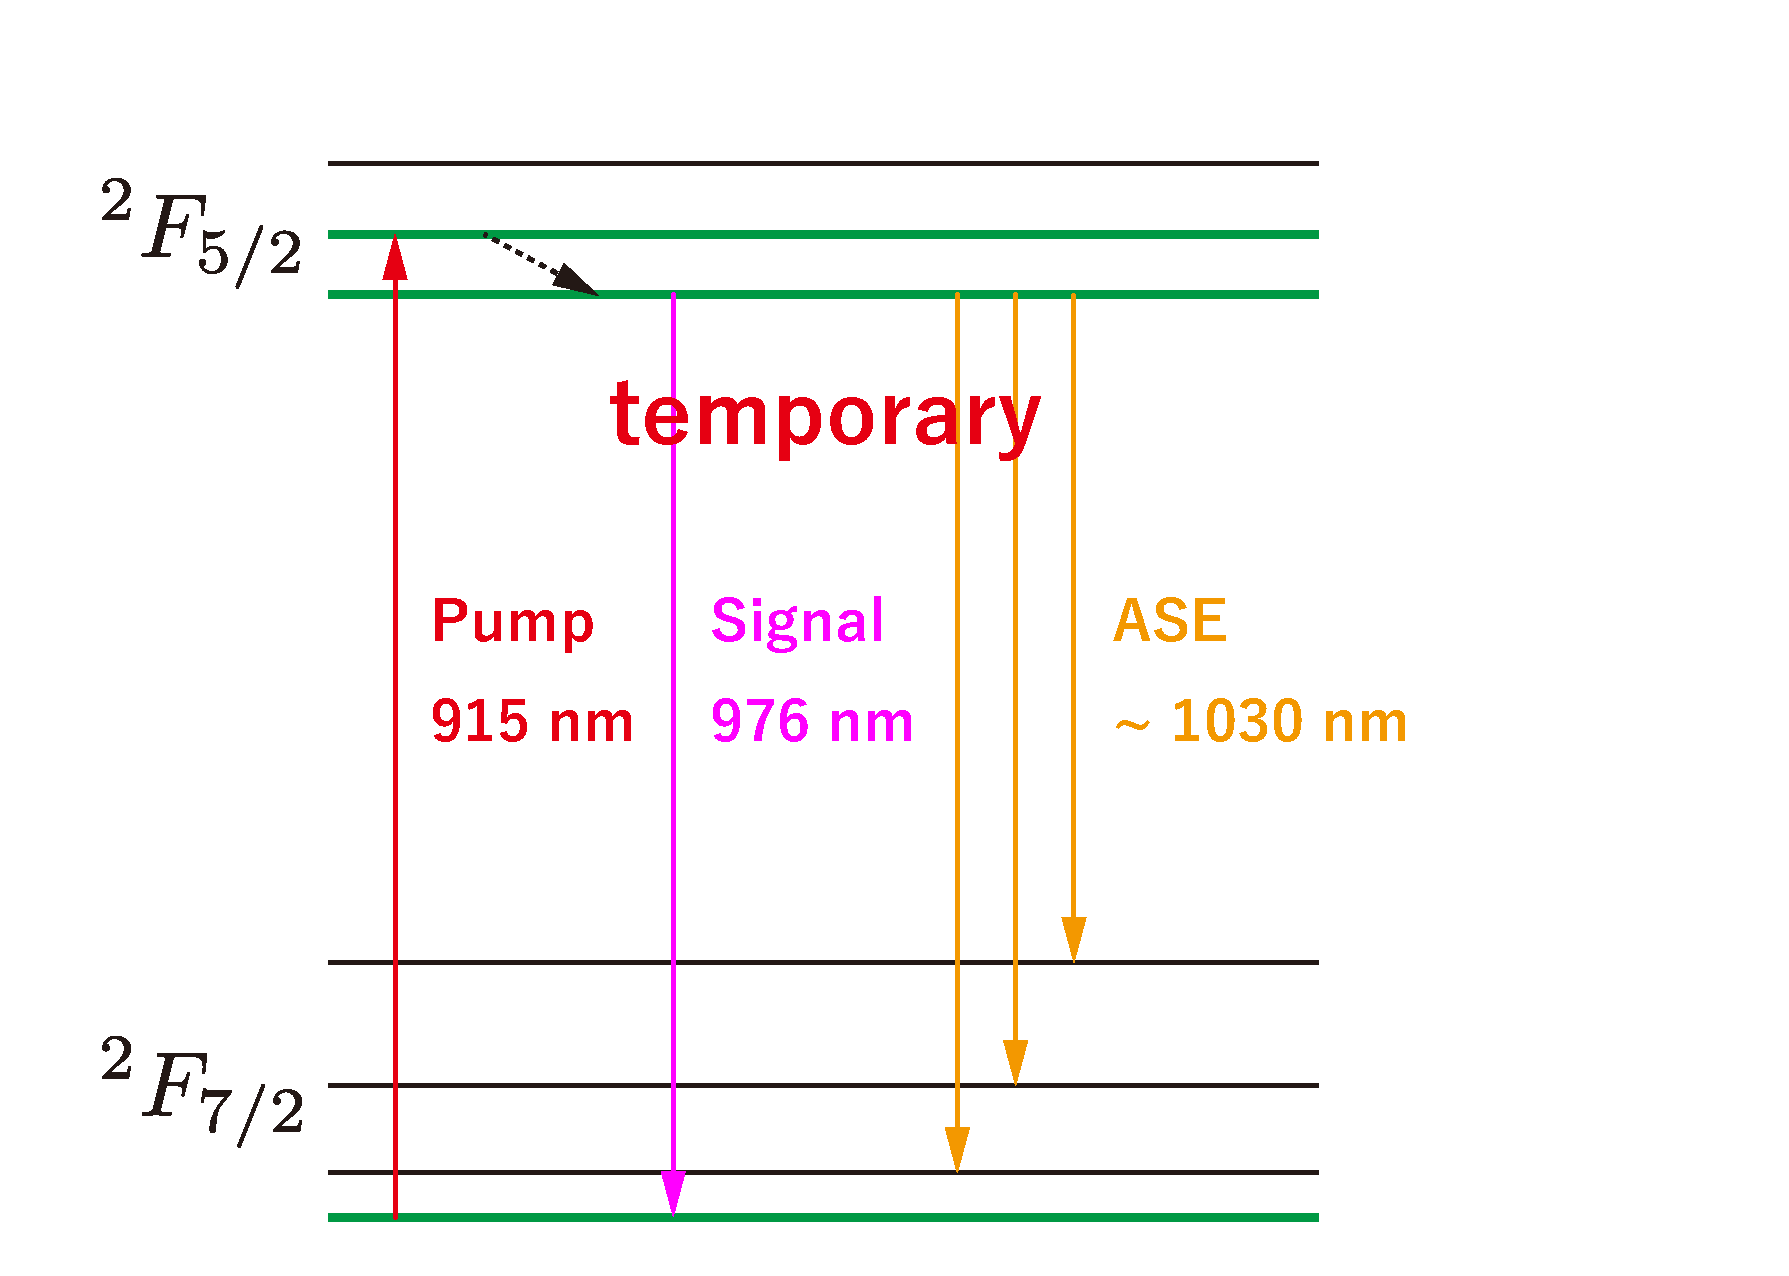
\includegraphics[keepaspectratio, width=0.9\linewidth]{./Figure/RelevantEnergyLevelOfYb3+InAluminosilicate}
    %\subcaption{}
  \end{minipage}
  \begin{minipage}[b]{0.5\linewidth}
    \centering
    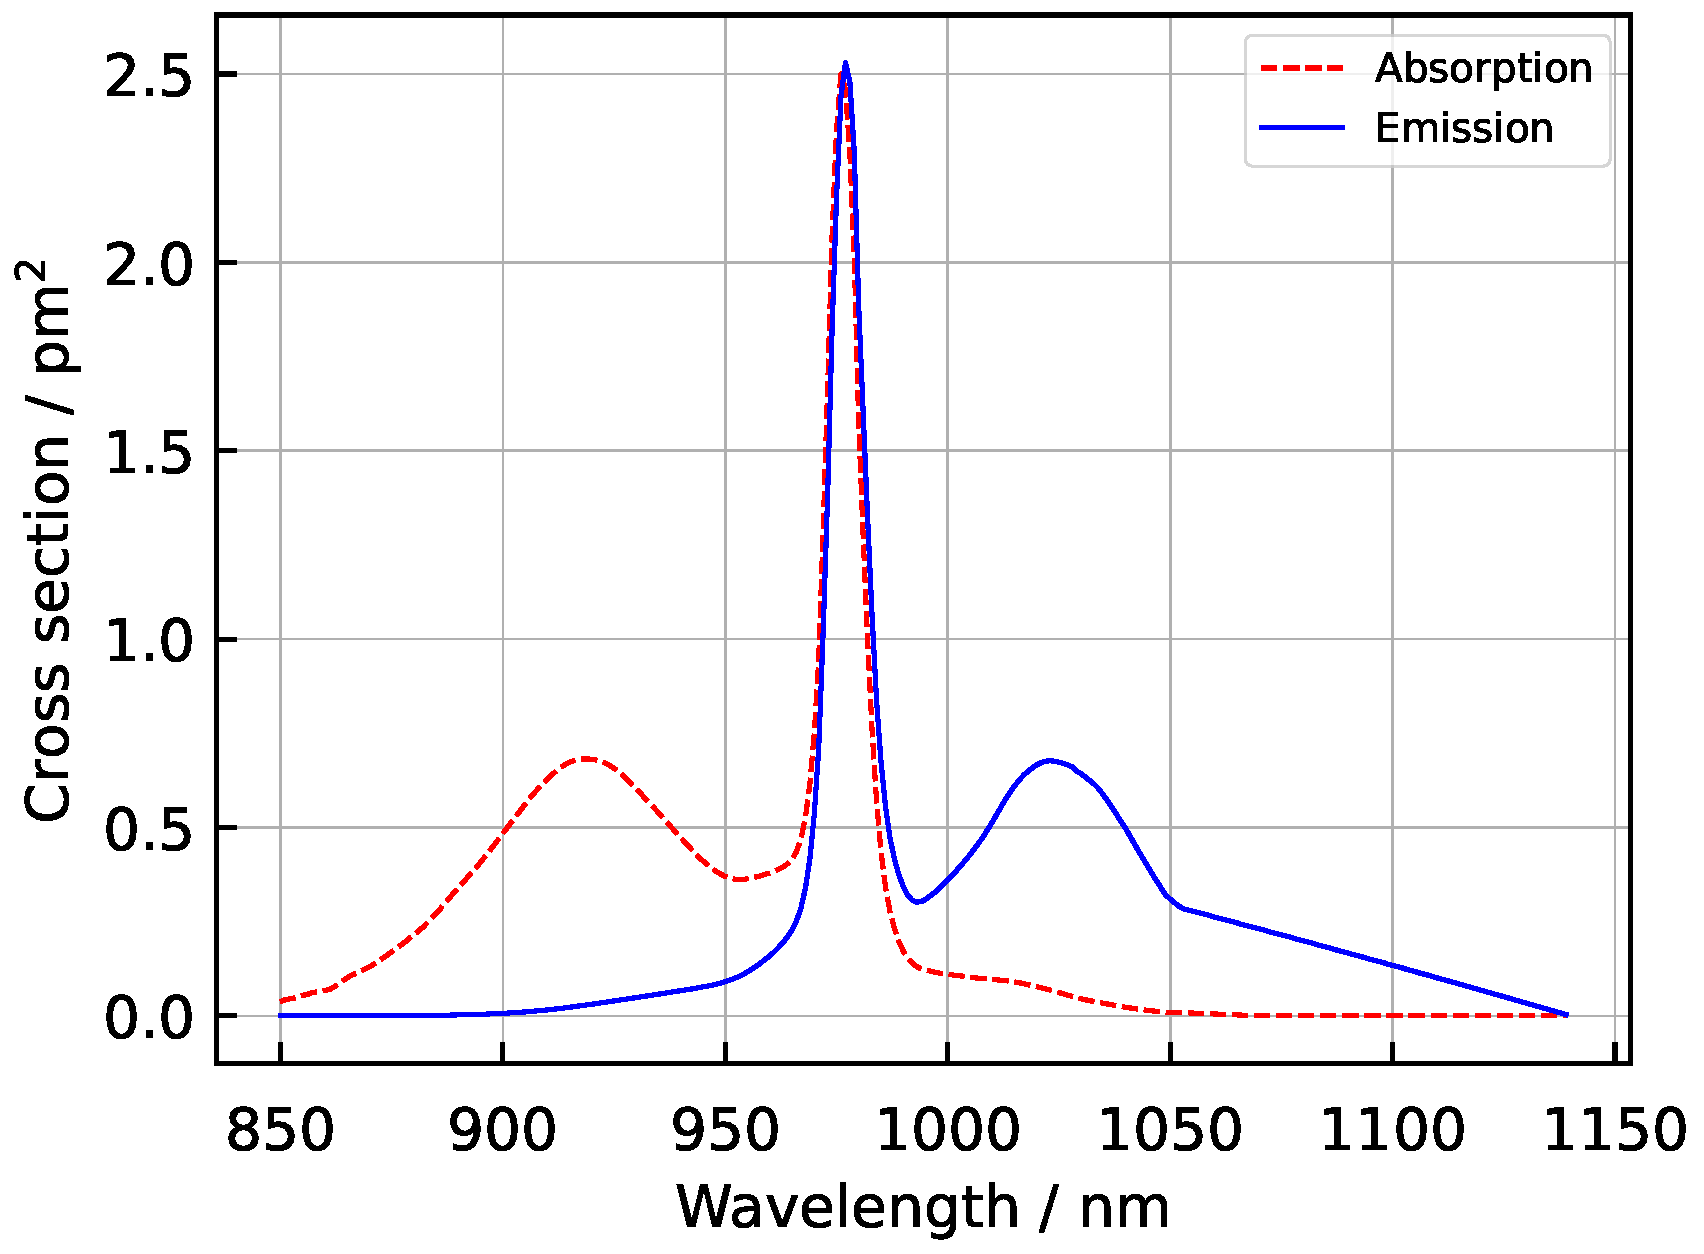
\includegraphics[keepaspectratio, width=0.9\linewidth]{./Figure/CrossSectionOfYb3+InAluminosilicate}
    %\subcaption{}
  \end{minipage}
  \caption{Relevant energy level and cross sections of Yb-doped fiber.}
  \label{fig:EnergylevelAndCrosssectionOfYb3+}
\end{figure}

Further estimation for amplifiers requires numerical simulation.
For the estimation of \SI{1112}{\nm}, only the $\mathrm{LP_{01}}$ mode should be considered as the propagation mode, while a several higher modes include in the calculation for the \SI{976}{\nm} amplifier because the few-mode fiber is used for the gain fiber.
From the normalizded frequency $V_{c}$ of ASE, we included a few higher-order modes of $\mathrm{LP_{01}}$, $\mathrm{LP_{11}}$, $\mathrm{LP_{21}}$, and $\mathrm{LP_{02}}$ for ASE calculation, while only $\mathrm{LP_{01}}$ mode was considered for signal calculation because the seed laser almost consisted of $\mathrm{LP_{01}}$ mode.
In addition, they are assumed that coupling between the $\mathrm{LP_{lm}}$ modes is negligible, and that Yb dopant are uniformly distributed throughout the fiber core.
Referring to \cite{gong2007numerical}, we developed the simulation code based on a model which has the cross section of the doped core devided into $M$ layers in the radial direction.
%The cross section of the doped core devided into $M$ layers in radial direction.
The rate equation and propagation equations for forward and backward propagating pump, signal, and ASE were given by
\begin{equation}
  \begin{split}
    N_{1k} + N_{2k} &= 1\\
    \dv{N_{2k}}{t} &= \frac{\lambda_{p} \Gamma_{p, k}}{hcA_{k}} (\sigma_{a}(\lambda_{p})N_{1k} - \sigma_{e}(\lambda_{p})N_{2k}) (P^{+}_{p} + P^{-}_{p})\\
    &+ \frac{\lambda_{s} \Gamma_{s, k}}{hcA_{k}} (\sigma_{a}(\lambda_{s})N_{1k} - \sigma_{e}(\lambda_{s})N_{2k}) (P^{+}_{s} + P^{-}_{s})\\
    &+ \frac{\lambda_{a} \Gamma_{a, k}}{hcA_{k}} (\sigma_{a}(\lambda_{a})N_{1k} - \sigma_{e}(\lambda_{a})N_{2k}) (P^{+}_{a} + P^{-}_{a}) - \frac{N_{2k}}{\tau},
  \end{split}
  \label{eq:RateEquation}
\end{equation}

\begin{align}
  \dv{P^{\pm}_{p}}{z} = &\pm \sum_{k}^{M} \Gamma_{p, k} (\sigma_{e}(\lambda_{p})N_{2k} - \sigma_{a}(\lambda_{p})N_{1k})NP^{\pm}_{p} \mp \alpha P^{\pm}_{p} \label{eq:PumpPropagationEquation}\\
  \dv{P^{\pm}_{s}}{z} = &\pm \sum_{k}^{M} \Gamma_{s, k} (\sigma_{e}(\lambda_{s})N_{2k} - \sigma_{a}(\lambda_{s})N_{1k})NP^{\pm}_{s} \mp \alpha P^{\pm}_{s} \label{eq:SignalPropagationEquation}\\
  \dv{P^{\pm}_{a, i}}{z} = &\pm \sum_{k}^{M} \Gamma_{a, k} (\sigma_{e}(\lambda_{a})N_{2k} - \sigma_{a}(\lambda_{a})N_{1k})NP^{\pm}_{a} \mp \alpha P^{\pm}_{a, i} \nonumber \\
  &\pm \sum_{k}^{M} m\sigma_{e}(\lambda_{a})\Gamma_{a, k, i} N_{2k}N \frac{hc^{2}}{\lambda_{a}^{3}} \Delta\lambda_{a}. \label{eq:ASEPropagationEquation}
\end{align}
Here $P^{\pm}_{j} (j = p, s, a)$ is the pump, signal, and ASE power, whose symbol of $\pm$ indicates to forward(+) and backward(-) propagation.
$\lambda_{j}$ is the wavelength of the pump, signal and ASE, $\sigma_{a}(\lambda_{j})$ and $\sigma_{e}(\lambda_{j})$ are the absorption and emission cross-sections of Yb ions at the wavelength $\lambda_{j}$, respectively.
$A_{k} = \pi(r_{k+1}^2 - r_{k}^{2}), (k = 0, 1, \cdots M-1))$ is the $k^{\mathrm{th}}$ layer area of the doped core, $N$ is the Yb-ion dopant density, $N_{1k}$ and $N_{2k}$ are the population of the ground and excited states at the $k^{\mathrm{th}}$ layer, respectively.
$\Gamma_{(p, s), k}$ is the overlapping factors for pump and signal, and $\Gamma_{a, k, i}$ is the overlapping factor of $i^{\mathrm{th}}$ transverse mode of the ASE relative to the $k^{\mathrm{th}}$ layer.
$\tau$ is the spontaneous lifetime of Yb ion in the excited state, and $\alpha_{j}$ and $\alpha_{j, i}$ are loss factors during fiber propagation.
$h$ is the plamck constant and $c$ is the speed of light in vacuum.

In this experiment, we set the boundary conditions for the above equations as following:
\begin{equation}
  \begin{split}
    P_{p, s}^{+}(0) &= P_{p, s} + R1P_{p, s}^{-}(0) \\
    P_{p, s}^{-}(L) &= P_{p, s} + R2P_{p, s}^{+}(L) \\
    P_{a, i}^{+}(0) &= R1P_{a, i}^{-}(0) \\
    P_{a, i}^{-}(L) &= R2P_{a, i}^{+}(0), \\
  \end{split}
\end{equation}
where $L$ is length of the doped fiber, and $R1$ and $R2$ are the equivalent reflectance at $z = 0$ and $z = L$ which includes reflections from outside the amplifier.
The simulation sequence is as follows:
(1) Using initial conditions and \cref{eq:RateEquation,eq:PumpPropagationEquation,eq:SignalPropagationEquation,eq:ASEPropagationEquation}, the evolution of the forward propagating pump, signal, and ASE powers from $z = 0$ to $z = L$ are calculated;
(2) The initial condition for backward propagation is derived from the each forward-propagation output at $z = L$, and the evolution of backward propagation is calculated in the reverse direction of the procedure (1);
(3) Then we repeat the steps (1) and (2) until the each forward propagation at $z = L$ and the backward propagation at $z = 0$ are converged.
Comparison of simulation and experimental results will be discussed in a later Section \ref{sec:Discussion}.


\section{Experimental setup}
\subsection{976\,nm amplifier system}

\begin{figure}[h!]
  \centering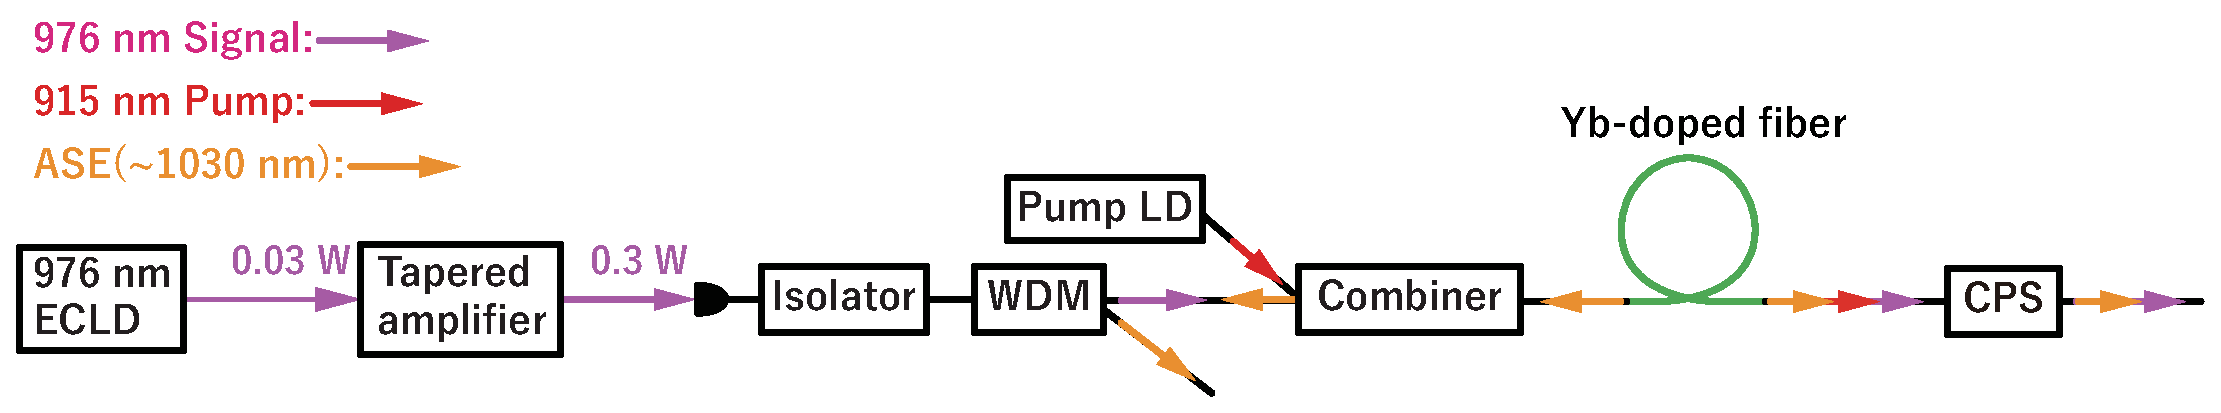
\includegraphics[width=\linewidth]{./Figure/976nmYDFASystem.eps}
  \caption{\SI{976}{\nm} YDFA system.}
  \label{fig:976YDFASystem}
\end{figure}
\todo{add model name of components}
A schematic of the \SI{976}{\nm} YDFA system is shown in Fig.~\ref{fig:976YDFASystem}.
An external-cavity laser diode(ECLD) at \SI{976}{\nm} followed a tapered amplifier(TA) is used as a seed laser.
The output of seed laser is pre-amplified by the TA up to nearly \SI{1}{\W}, and coupled to the YDFA input which is a polarization maintaining(PM) fiber with a FC/APC connector.
Owing to the spatial-mode mismatch of the output from TA, the power coupled to the input is only \SI{300}{\mW}.
The input of YDFA is fusion-spliced to an inline isolator and a wavelength division multiplexing(WDM) filter, which protect the seed laser from backward propagation light generated in a gain fiber.
The WDM which has three ports: a common port, a pass port, and a reflection port separates ASE around \SI{1020}{\nm} from signal path(common-pass) to the reflection port.
A fiber end of the reflection port is cleaved so that it is angled at least \ang{8} in order to prevent ASE from returning from the end to a gain fiber.
A \SI{915}{\nm} pump radiation is generated from fiber-coupled laser diode with output power of up to \SI{70}{\W}.
The pump laser is fixed on a water-cooled heatsink for stable operation.
A signal pump combiner, which has a signal port with PM fiber of \SI{6/125}{\um}, two pump ports with multimode fibers of \SI{105/125}{\um}, and a common port with double-cladding PM fiber of \SI{20/125}{\um}, combines the seed laser and the pump laser into the common port fiber.
The Yb-doped fiber fusion-spliced from the common port fiber of the combiner is rolled to approximately \SI{100}{\mm} in diameter and fixed on a water-cooled heatsink with a thermal conductive sheet.
For safe operation of the YDFA, all the bare glass cladding around the fusion-spliced points are recoated with low-refractive index polymer.
A residual pump power in the output of the Yb-doped fiber is removed by a cladding power stripper(CPS).
Amplified signal and ASE are collimated by pigtailed collimator, separated by a filter, and measured by power meters, respectively.


\subsection{1112\,nm amplifier system}

\begin{figure}[h!]
  \centering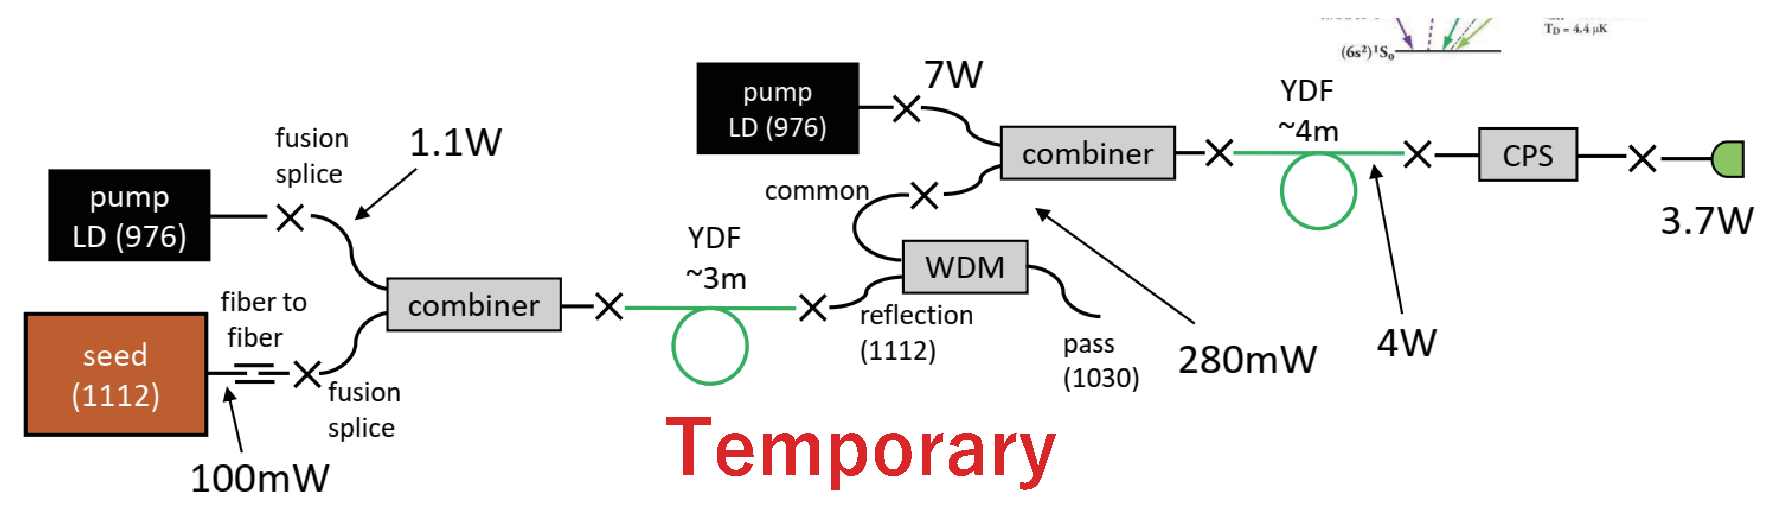
\includegraphics[width=\linewidth]{./Figure/1112nmYDFASystem_Temp.eps}
  \caption{\SI{1112}{\nm} YDFA system.}
  \label{fig:1112YDFASystem}
\end{figure}

A schematic of the \SI{1112}{\nm} YDFA system is shown in Fig.~\ref{fig:1112YDFASystem}.
The \SI{1112}{\nm} YDFA system is composed of a seed laser and two amplifiers.
A fiber laser at \SI{1112}{\nm}(Menlo systems Orange one-2) is used as the seed laser.
The output singlemode fiber with a FC/APC connector is contacted to the input singlemode fiber of the first stage amplifier with a mating sleeve.
A coupled power into the input is about \SI{80}{\mW}.
As pump lasers, a \SI{976}{\nm} fiber-coupled diode laser installed on an air-cooled heatsink with maximum output of \SI{7}{\W} is used for the first and second stage, respectively.
The configuration of the first stage amplifier is similar to the \SI{976}{\nm} system except fiber type.
The seed laser and the pump laser are combined into a double-cladding fiber of \SI{10/125}{\um} by a pump-signal combiner.
The first Yb-doped fiber is under no temperature control because the pump power is limited to less than \SI{1}{\W}.
Before a second pump-signal combiner, the ASE around \SI{1020}{\nm} generated in first Yb-doped fiber is removed by a WDM.
The \SI{1112}{\nm} signal after the second combiner is \SI{220}{\mW}.
The second Yb-doped fiber is rolled in a diameter of \SI{100?}{\mm}, and fixed inside an aluminum enclosure with thermal conductive sheet.
Temperature of the aluminum enclosure is controlled by peltier devices.
Similar to \SI{976}{\nm} system, the output of the second Yb-doped fiber is removed by CPS and collimated by pigtailed collimator.
The output power of the \SI{1112}{\nm} signal and the ASE near \SI{1020}{\nm} are obtained by measuring the output powers through long-pass filters with cut-on wavelengths at \SI{1100?}{\nm}.

\section{Experimental results}
\subsection{976\,nm YDFA}

\begin{figure}[h!]
  \begin{minipage}[b]{0.5\linewidth}
    \centering
    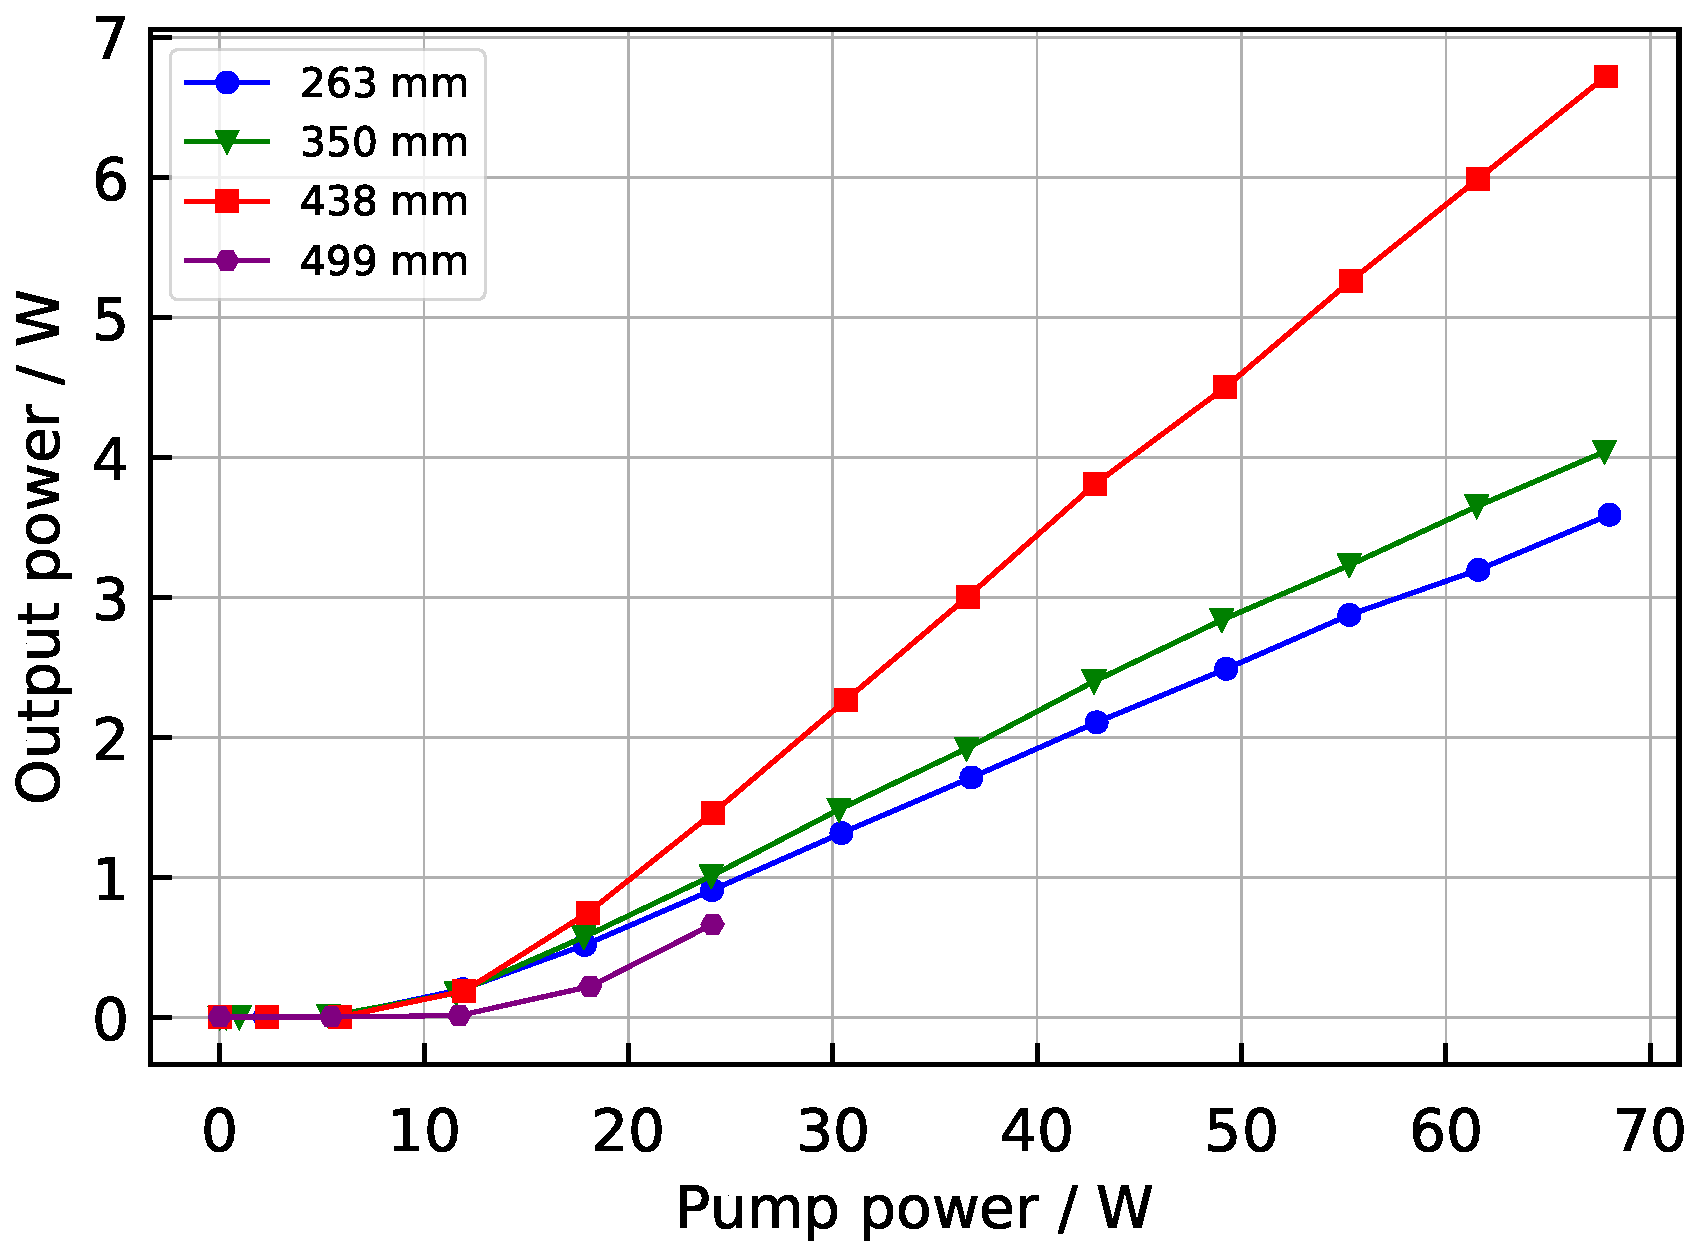
\includegraphics[keepaspectratio, width=0.9\linewidth]{./Figure/Yb1200-20-125DC-PM_SignalComparisonByLength_915Pump976Seed_Exp}
    \subcaption{}
  \end{minipage}
  \begin{minipage}[b]{0.5\linewidth}
    \centering
    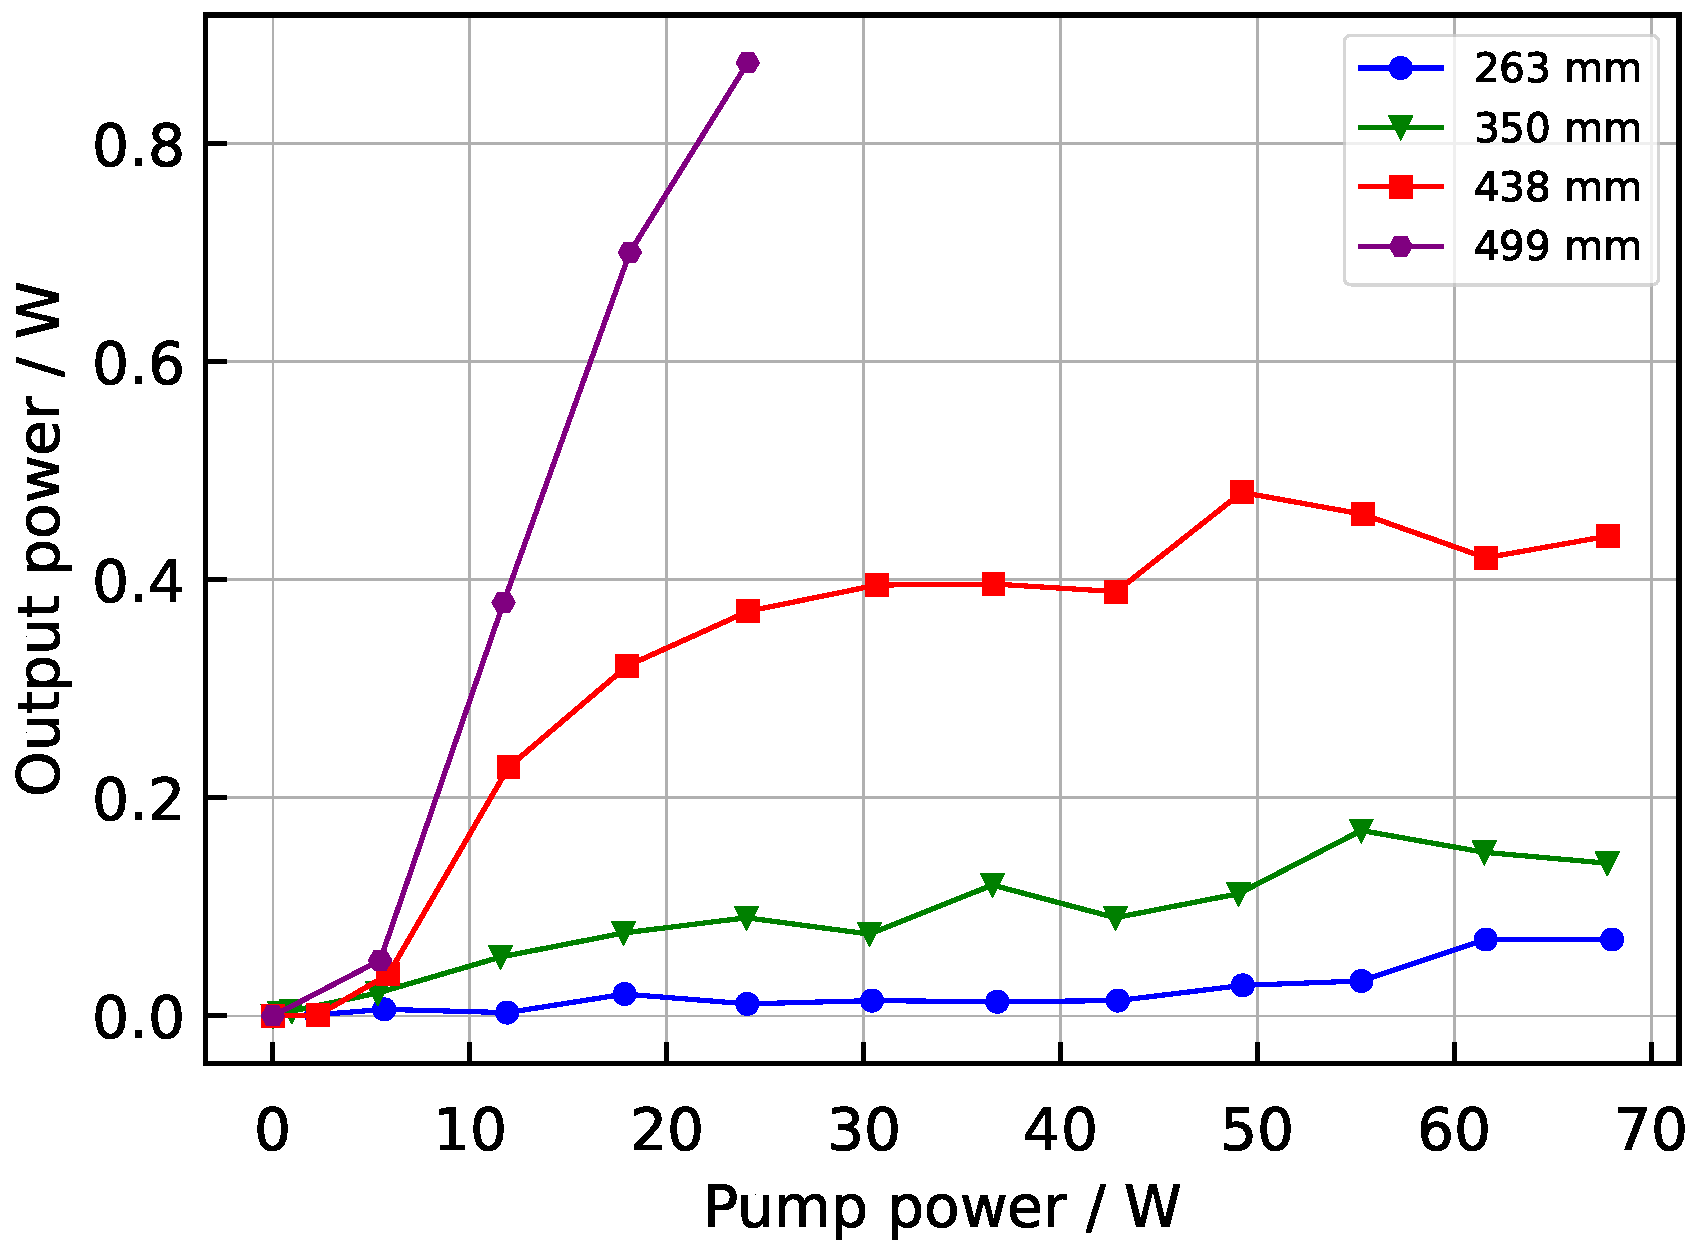
\includegraphics[keepaspectratio, width=0.9\linewidth]{./Figure/Yb1200-20-125DC-PM_ASEComparisonByLength_915Pump976Seed_Exp}
    \subcaption{}
  \end{minipage}
  \caption{Measured \SI{976}{\nm} and ASE around \SI{1020}{\nm} power as a function of the launched \SI{915}{\nm} pump power.}
  \label{fig:OutputComparisonOfNLIGHT976YDFA}
\end{figure}

The \SI{976}{\nm} and ASE near \SI{1020}{\nm} output power of the YDFA are shown in Fig.~\ref{fig:OutputComparisonOfNLIGHT976YDFA}.
In this measurement, we used a Yb-doped aluminosilicate fiber(nLIGHT, Yb1200-20/125DC-PM) as a gain fiber.
We tested the \SI{263}{\mm}, \SI{350}{\mm}, \SI{438}{\mm}, and \SI{499}{\mm} long Yb-doped fibers at pump powers up to about \SI{70}{\W}.
As increasing the length of the Yb-doped fiber, the \SI{976}{\nm} output power increases, and reaches maximum at the \SI{438}{\mm} long fiber.
The \SI{976}{\nm} output increased with pump power to exceed the gain of \SI{1}{\dB} at \SI{12}{\W} pump power, and \SI{6.7}{\W} was achieved at \SI{68}{\W} pump power with a slope efficiency of 0.12.
The maximum \SI{976}{\nm} gain corresponds to \SI{14.5}{\dB}.
The reason for the lower slope efficiency compared to YDFAs which has operating wavelength above \SI{1}{\um} is that the \SI{976}{nm} transition occurs between the lowest sublevel of the ground state and the lowest sublevel of the excited state in Yb ion.
The ASE also increased with pump power above \SI{6}{\W}, but remained almost constant of \SI{0.4}{\W} above \SI{30}{\W} pump power.
In the test of \SI{499}{\mm} fiber, we applied the pump power less than \SI{25}{\W} because the ASE power significantly increased.

\begin{figure}[h!]
  \centering
  \begin{minipage}[b]{0.5\linewidth}
    \centering
    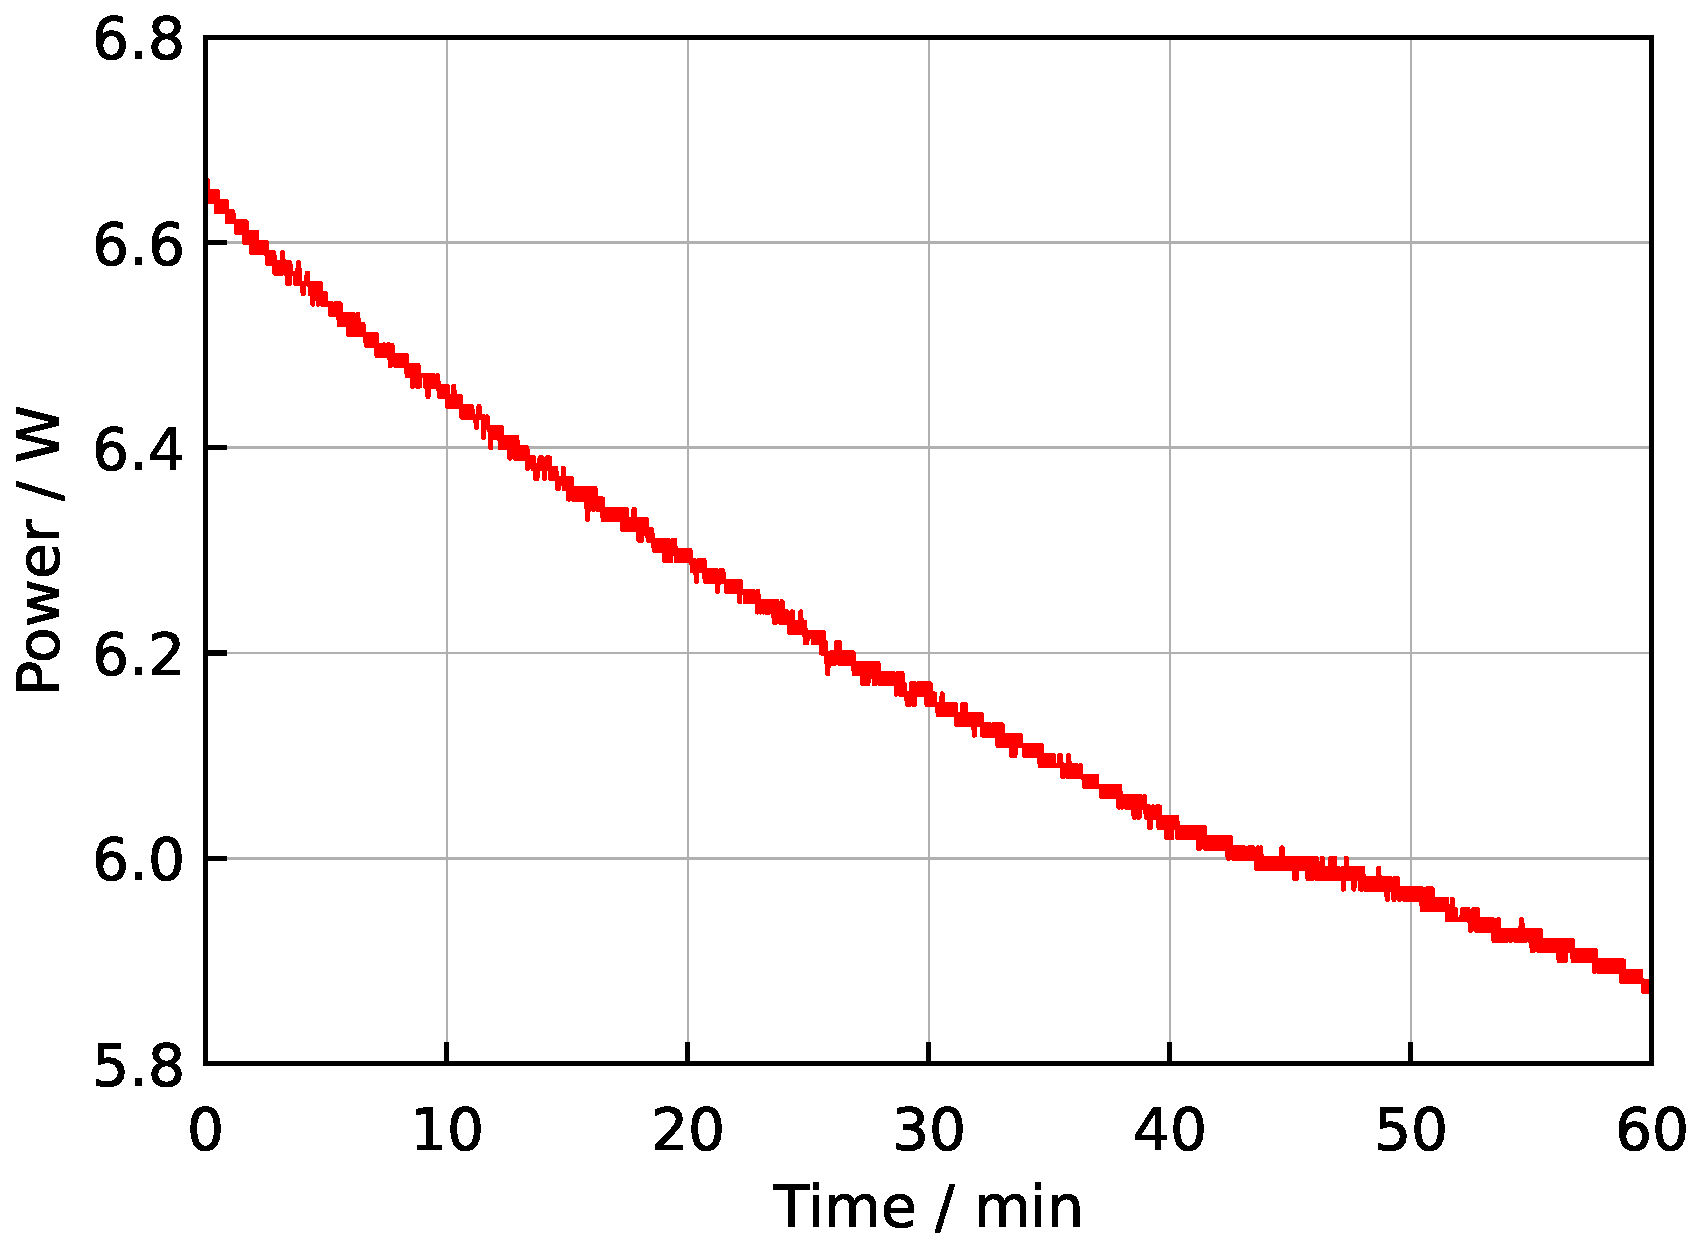
\includegraphics[keepaspectratio, width=0.9\linewidth]{./Figure/Yb1200-20-125DC-PM438mm_LongTermStability_915Pump70W976Seed0.24W_Exp}
    % \subcaption{}
  \end{minipage}
  \caption{The output power of the \SI{976}{\nm} YDFA with during \SI{60}{\minute}.}
  \label{fig:LongTermStabilityOfNLIGHT976YDFA}
\end{figure}
To measure the output stability of the \SI{976}{nm} YDFA, we logged the maximum output of the \SI{438}{mm} long fiber during \SI{60}{\minute}.
As the result shown in Fig.~\ref{fig:LongTermStabilityOfNLIGHT976YDFA}, the output of YDFA decayed in time to decrease by 12\% of its original power after \SI{60}{\minute}.
This is mainly due to photodarkening caused by the high-inversion distribution of Yb ion \cite{paschotta1997lifetime}.
Although the photodarkening is not fully understood, there are many proposals to mitigate the effect \cite{manek-honninger2007photodarkening, zhao2019elimination, engholm2008preventing}.
We developed another \SI{976}{\nm} YDFA using a Yb-doped fiber with phosphosilicate-glass core(Coractive, DCF-YB-20/128P-FAC).
\begin{figure}[h]
  \begin{minipage}[b]{0.5\linewidth}
    \centering
    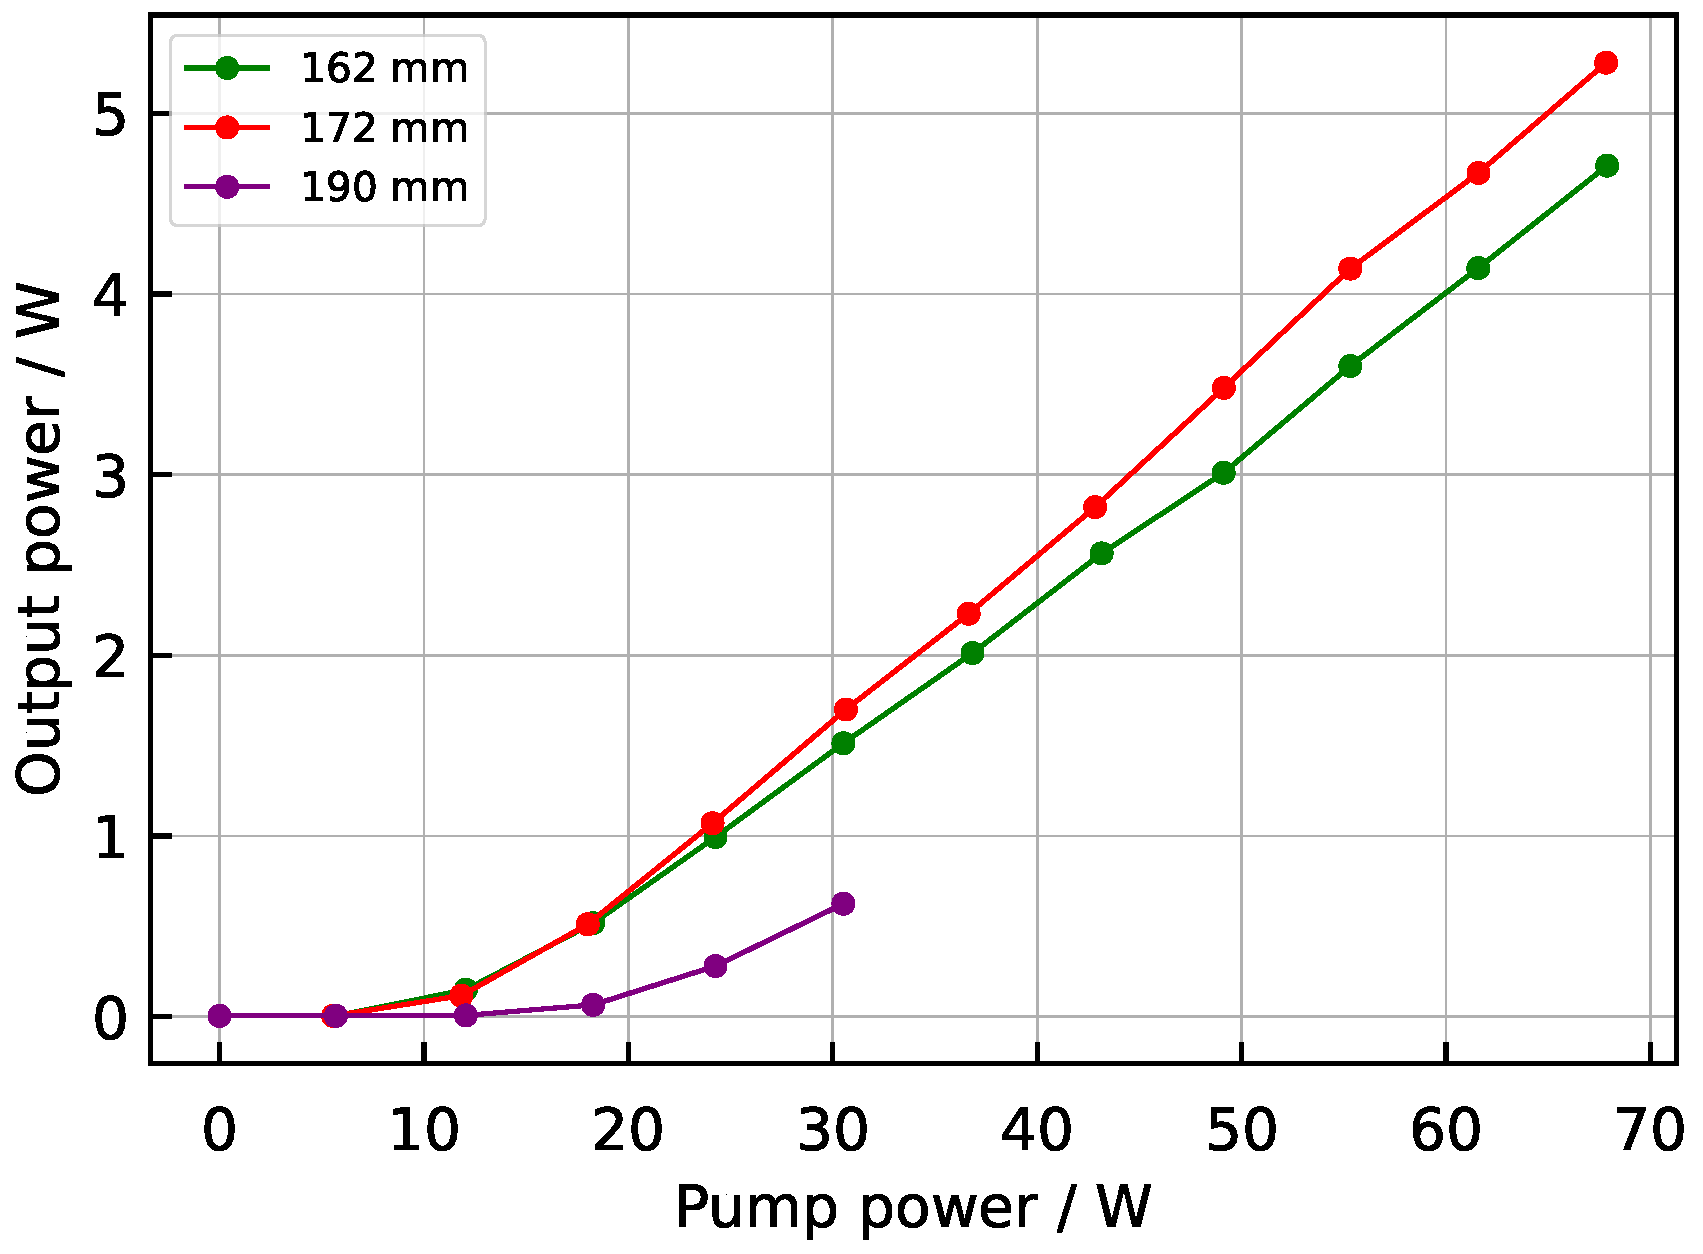
\includegraphics[keepaspectratio, width=0.9\linewidth]{./Figure/DCF-YB-20-128P-FAC172mm_SignalComparisonByLength_915Pump976Seed0.24W_Exp}
    \subcaption{}
  \end{minipage}
  \begin{minipage}[b]{0.5\linewidth}
    \centering
    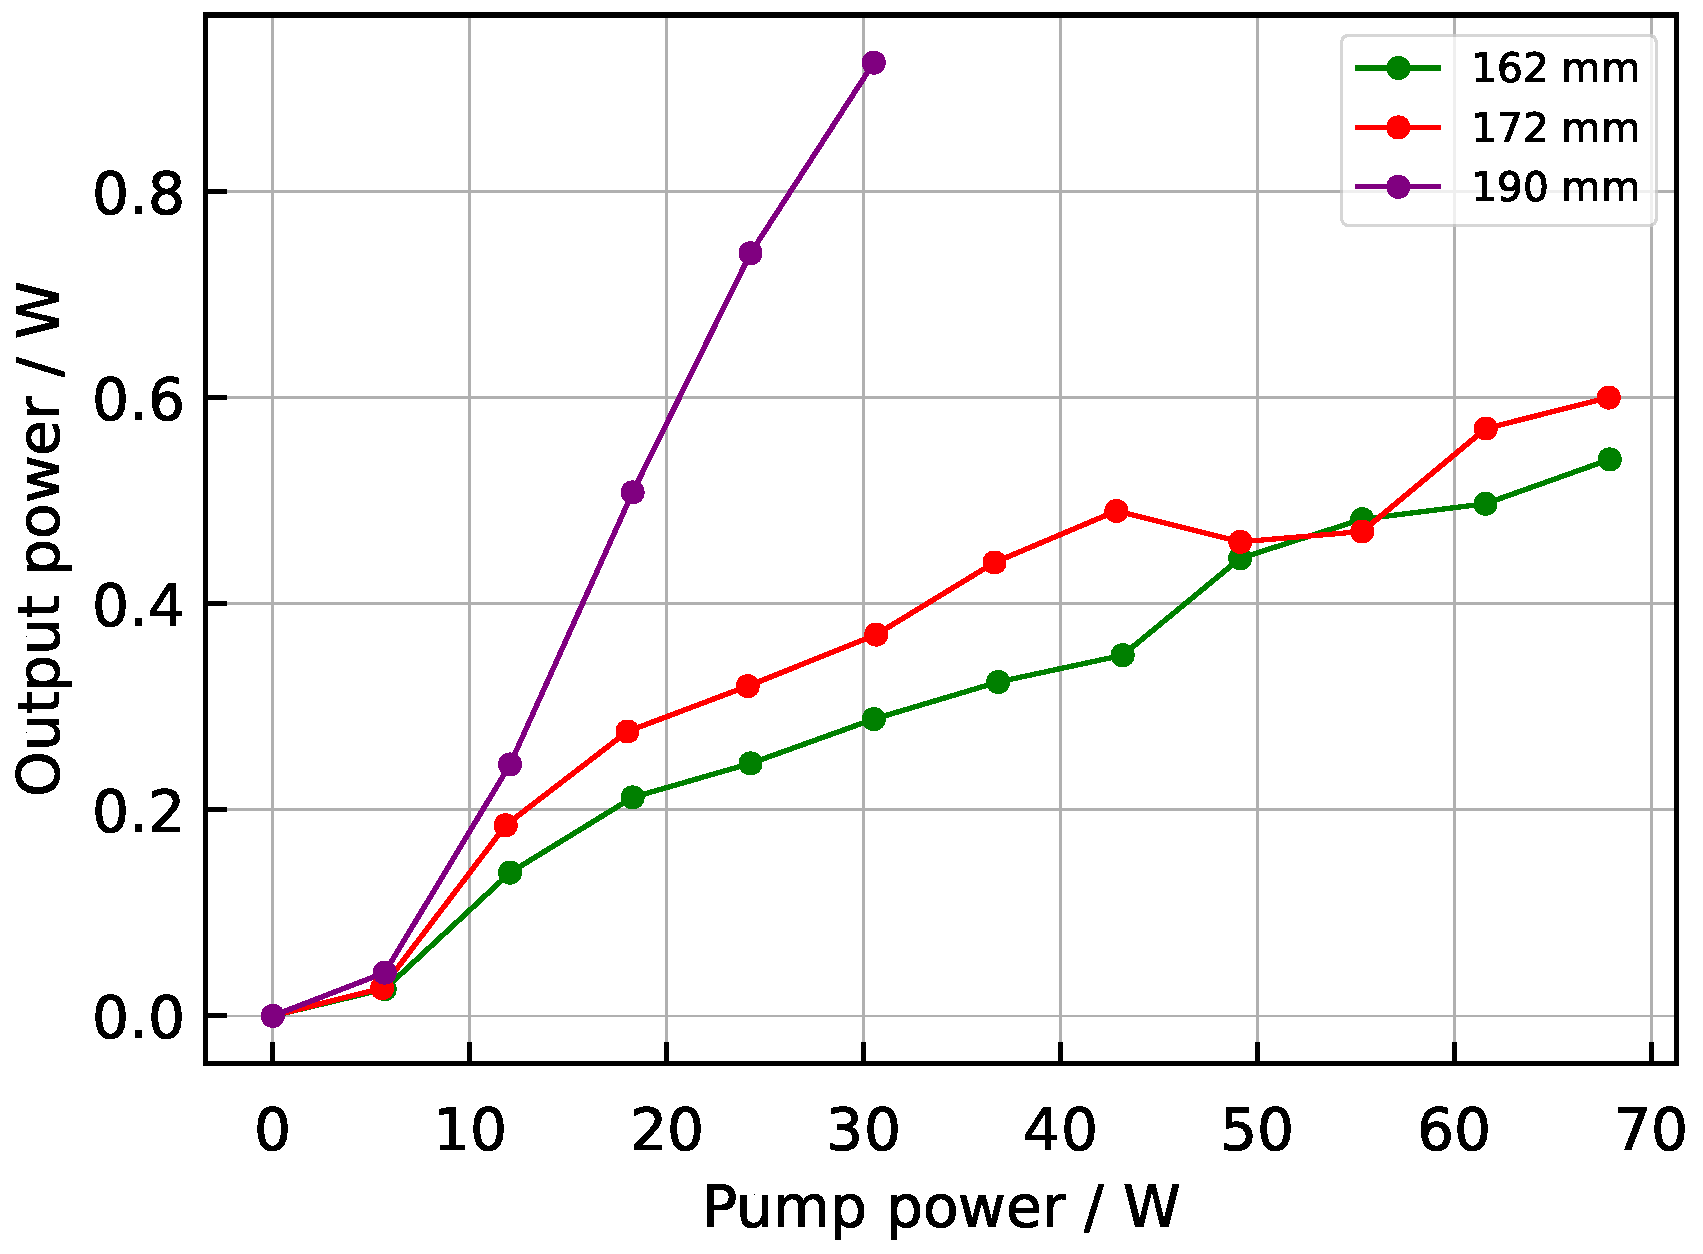
\includegraphics[keepaspectratio, width=0.9\linewidth]{./Figure/DCF-YB-20-128P-FAC172mm_ASEComparisonByLength_915Pump976Seed0.24W_Exp}
    \subcaption{}
  \end{minipage}
  \caption{Measured \SI{976}{\nm} and ASE around \SI{1020}{\nm} power as a function of the launched \SI{915}{\nm} pump power.}
  \label{fig:OutputComparisonOfCORACTIVE976YDFA}
\end{figure}
The output powers with the \SI{162}{\mm}, \SI{172}{\mm}, and \SI{190}{\mm} long phosphosilicate fibers are shown in the Fig.~\ref{fig:OutputComparisonOfCORACTIVE976YDFA}.
Both the \SI{976}{nm} amplified signal and the ASE increased with pump power and reached a maximum of \SI{5.3}{\W} and \SI{0.6}{\W} at pump power of \SI{68}{\W} with the \SI{172}{\mm} long fiber, respectively.
As with the case of the aluminosilicate fiber, the \SI{976}{\nm} output power was recorded with a duration of \SI{60}{\minute}.
The fluctuation of output was less than 1.5\% as shown in Fig.~\ref{fig:LongTermPowerStabilityOfCORACTIVE976YDFA}, which indicates that photo darkening is significantly reduced.


\begin{figure}[h!]
  \centering
  \begin{minipage}[b]{0.5\linewidth}
    \centering
    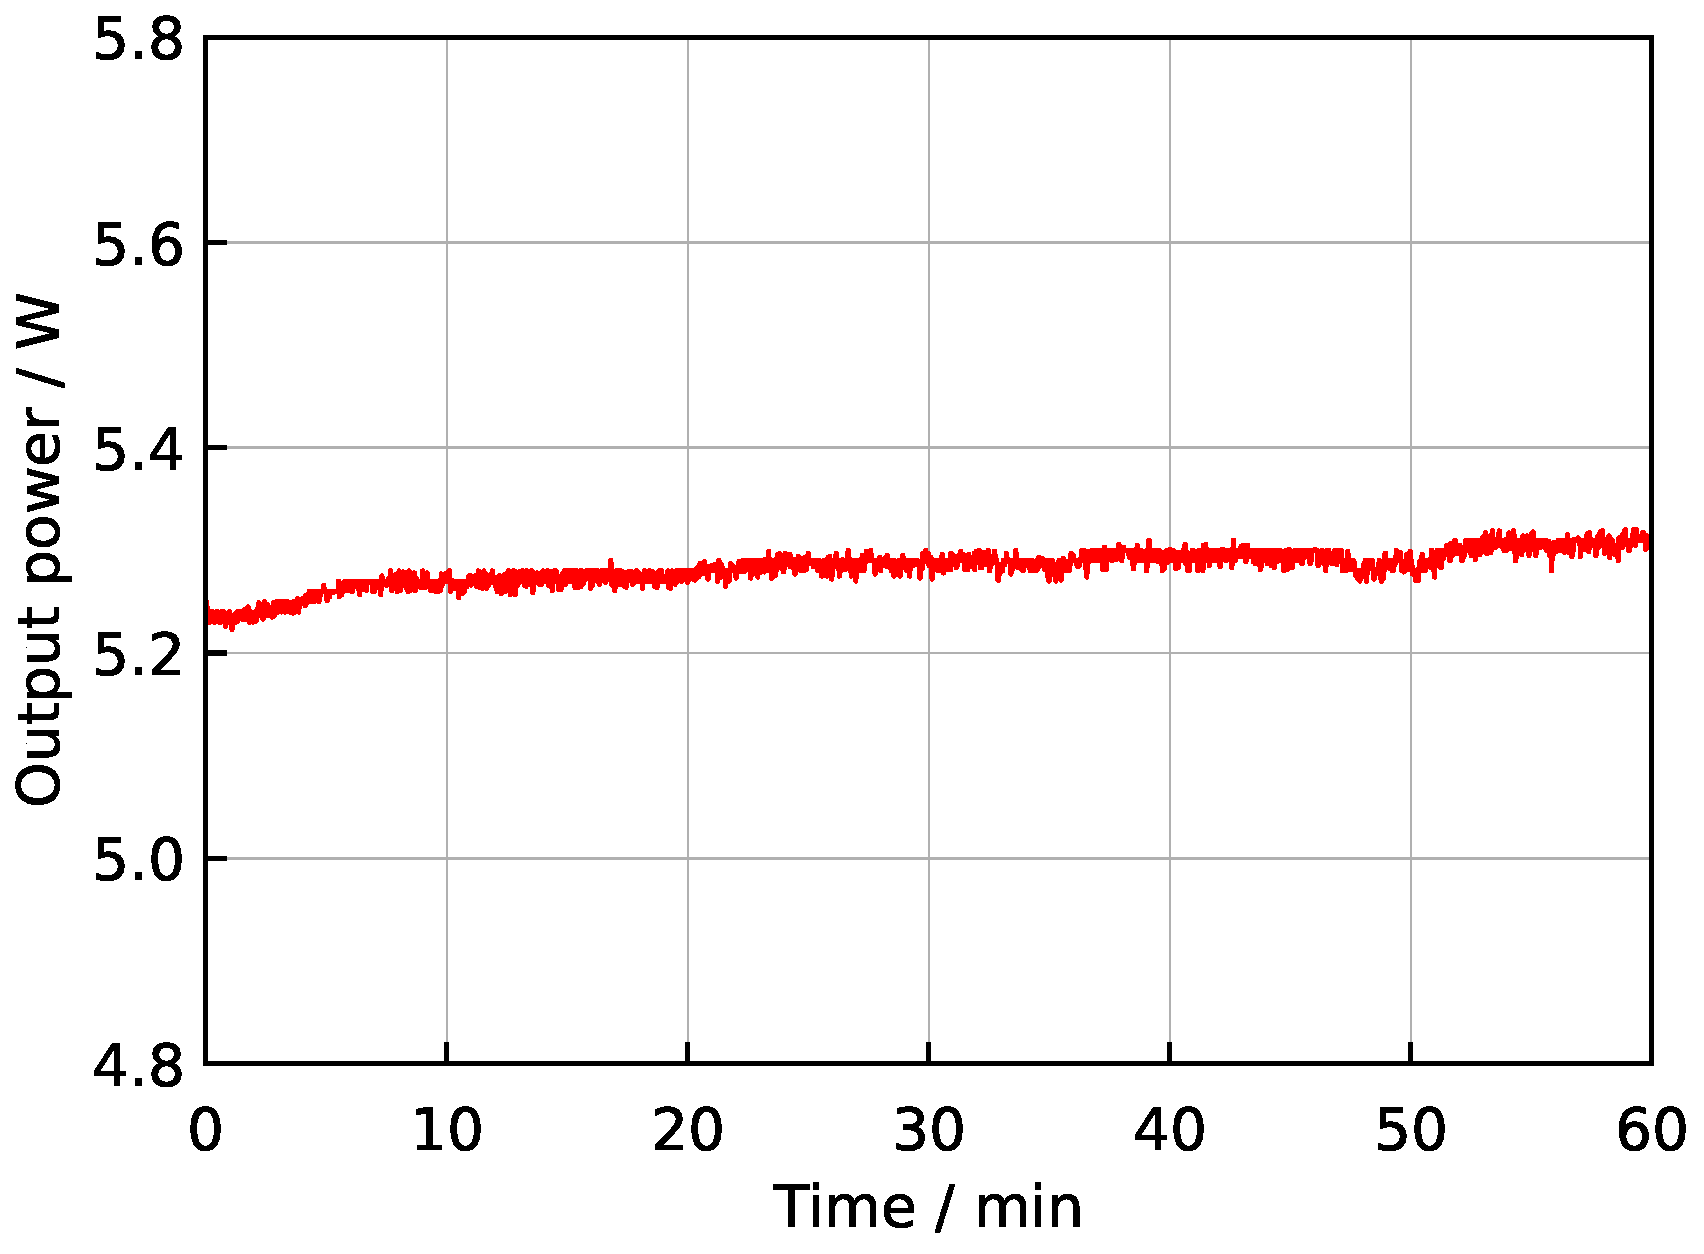
\includegraphics[keepaspectratio, width=0.9\linewidth]{./Figure/DCF-YB-20-128P-FAC172mm_SignalLongTermStability_915Pump70W976Seed0.24W_Exp.pdf}
    % \subcaption{}
    % \label{fig:LongTermPowerStabilityOfCORACTIVE976YDFA}
  \end{minipage}
  \caption{The output power stability of the \SI{976}{\nm} YDFA during \SI{60}{\minute}.}
  \label{fig:LongTermPowerStabilityOfCORACTIVE976YDFA}
\end{figure}

\subsection{1112\,nm YDFA}
\begin{figure}[h]
  \begin{minipage}[b]{0.5\linewidth}
    \centering
    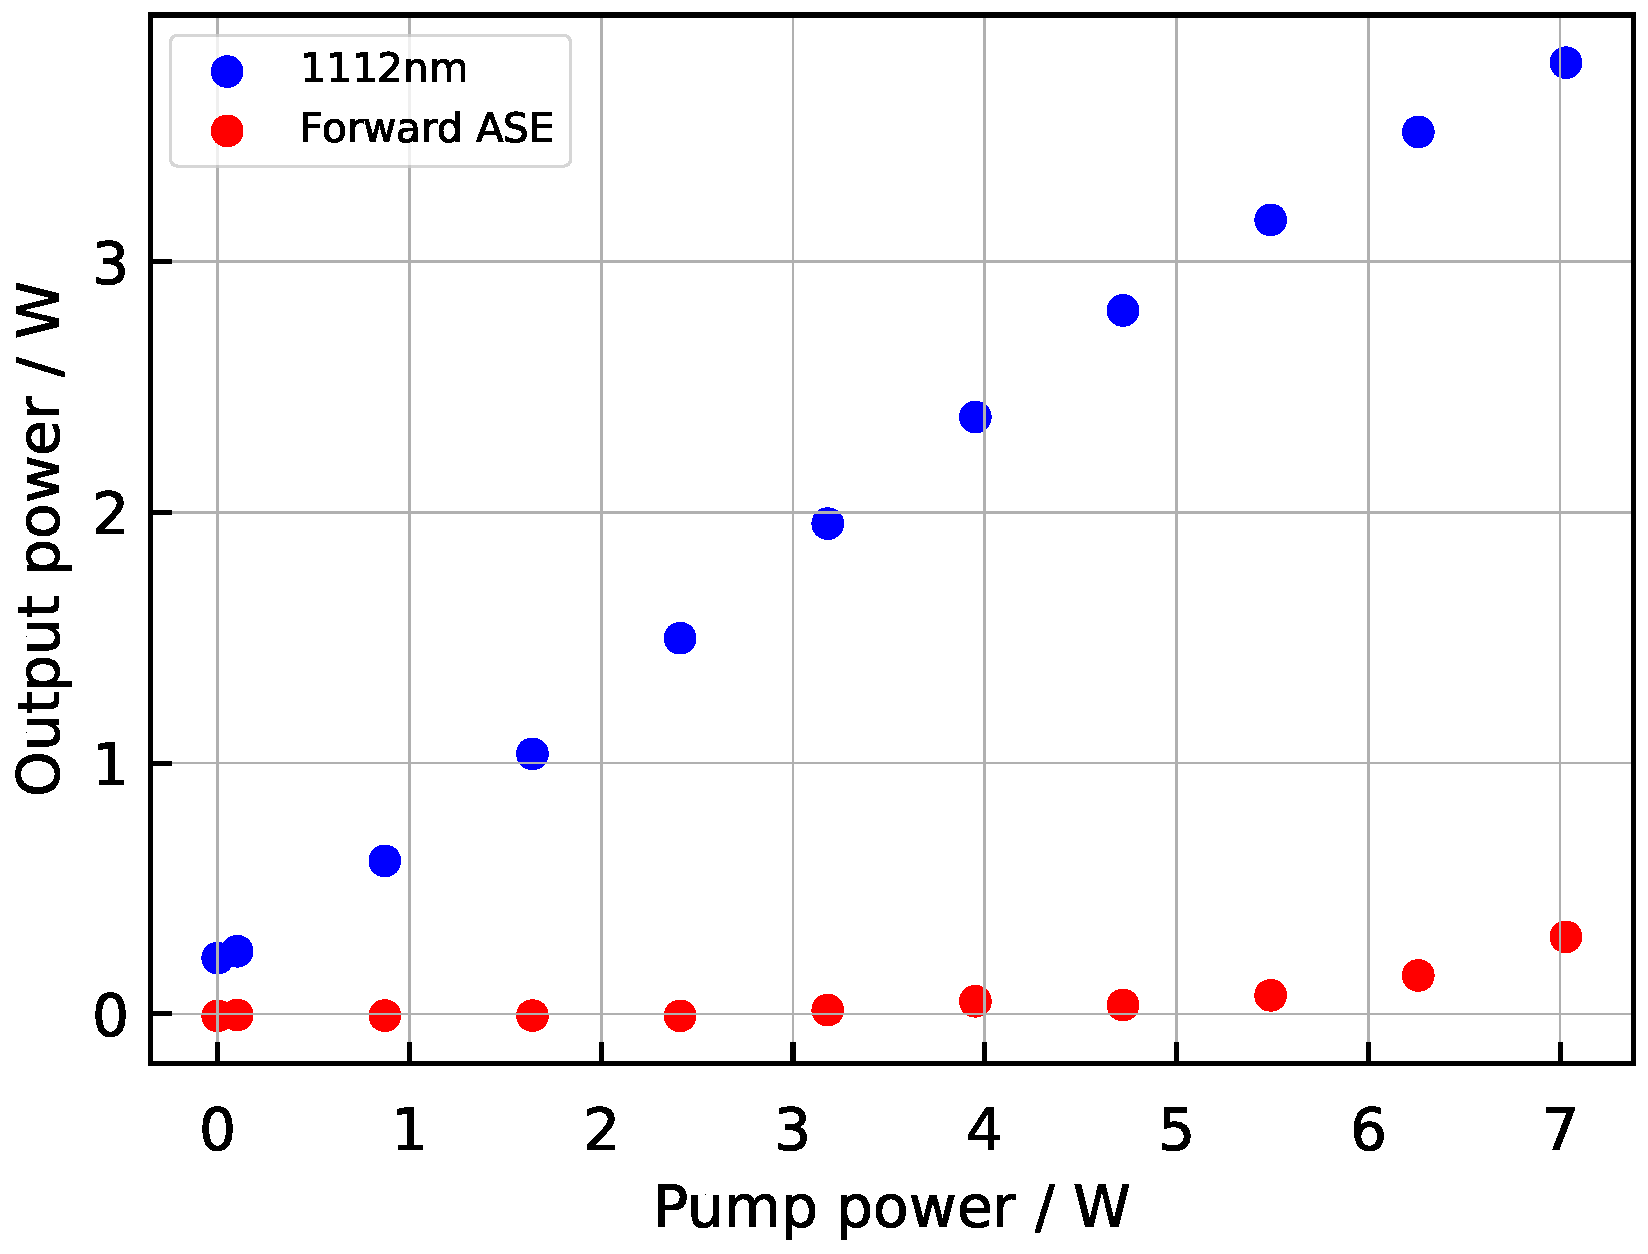
\includegraphics[keepaspectratio, width=0.9\linewidth]{./Figure/1112nmYDFA2ndStageOutput_Exp.pdf}
    \subcaption{}
    \label{fig:OutputOf1112YDFA}
  \end{minipage}
  \begin{minipage}[b]{0.5\linewidth}
    \centering
    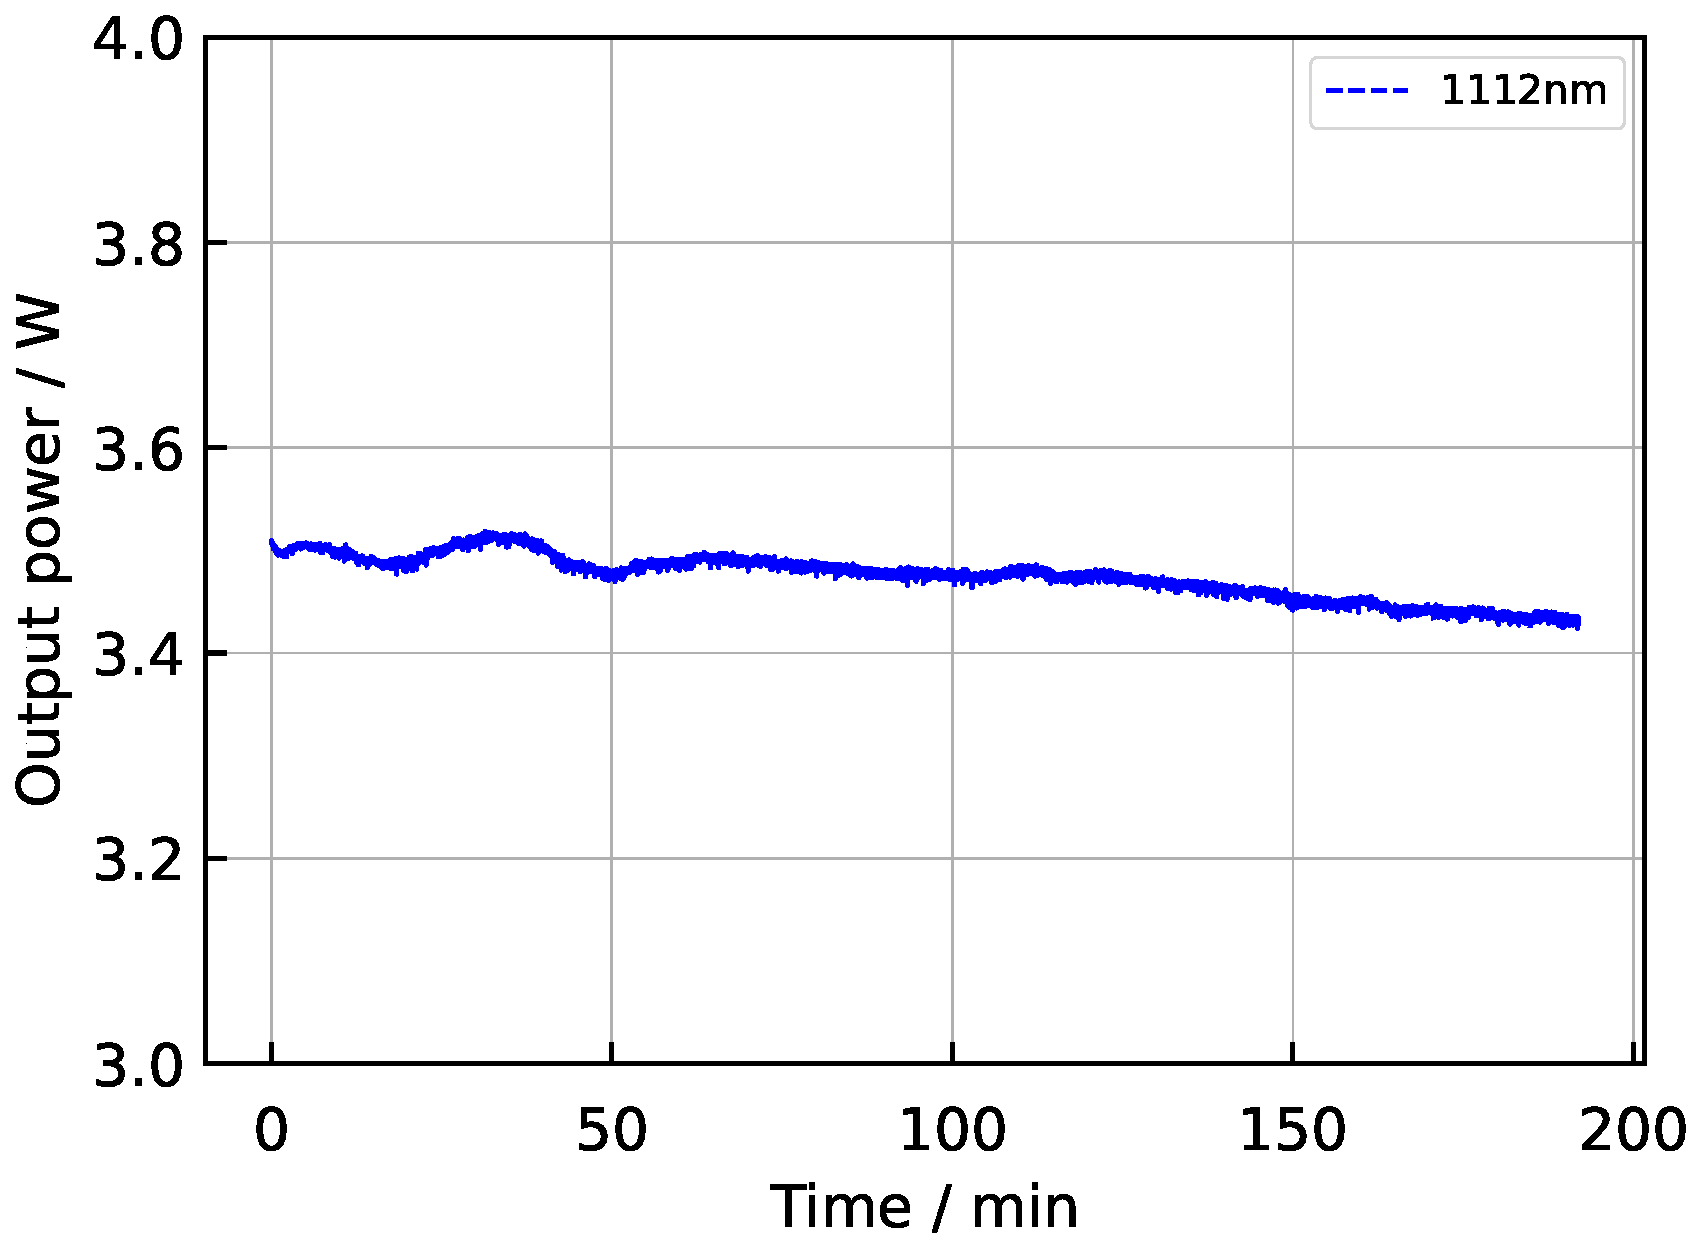
\includegraphics[keepaspectratio, width=0.9\linewidth]{./Figure/1112nmYDFA2ndStageOutputStability.pdf}
    \subcaption{}
    \label{fig:StabilityOf1112YDFA}
  \end{minipage}
  \caption{The output of \SI{1112}{\nm} YDFA. \subref{fig:OutputOf1112YDFA} The \SI{1112}{nm} and forward ASE as a function of the \SI{976}{\nm} pump power applied to the second stage amplifier. \subref{fig:StabilityOf1112YDFA} The \SI{1112}{\nm} output stability in duration over \SI{3}{\hour}.}
\end{figure}
In the \SI{1112}{\nm} YDFA, we used a Yb-doped fiber with a core based on aluminosilicate glass(nLIGHT, Yb1200-10/125DC) as a gain fiber.
The \SI{3}{\m} and \SI{4}{\m} long gain fiber are embedded in the first-stage and second-stage amplifiers, respectively.
Plots of the amplified \SI{1112}{nm} and forward ASE as a function of pump power applied to the second-stage amplifier are shown in Fig.~\ref{fig:OutputOf1112YDFA}.
The maximum generation of \SI{1112}{\nm} is \SI{3.8}{\W} at applied pump power of \SI{7}{\W}, which corresponds to the gain of \SI{12.3}{\dB}.
As shown in Fig.~\ref{fig:StabilityOf1112YDFA}, the variation of \SI{1112}{\nm} is less than 2.4\%.

\section{Comparison between numerical simulations and experimental results} \label{sec:Discussion}
\begin{figure}[h!]
  \begin{minipage}[b]{0.5\linewidth}
    \centering
    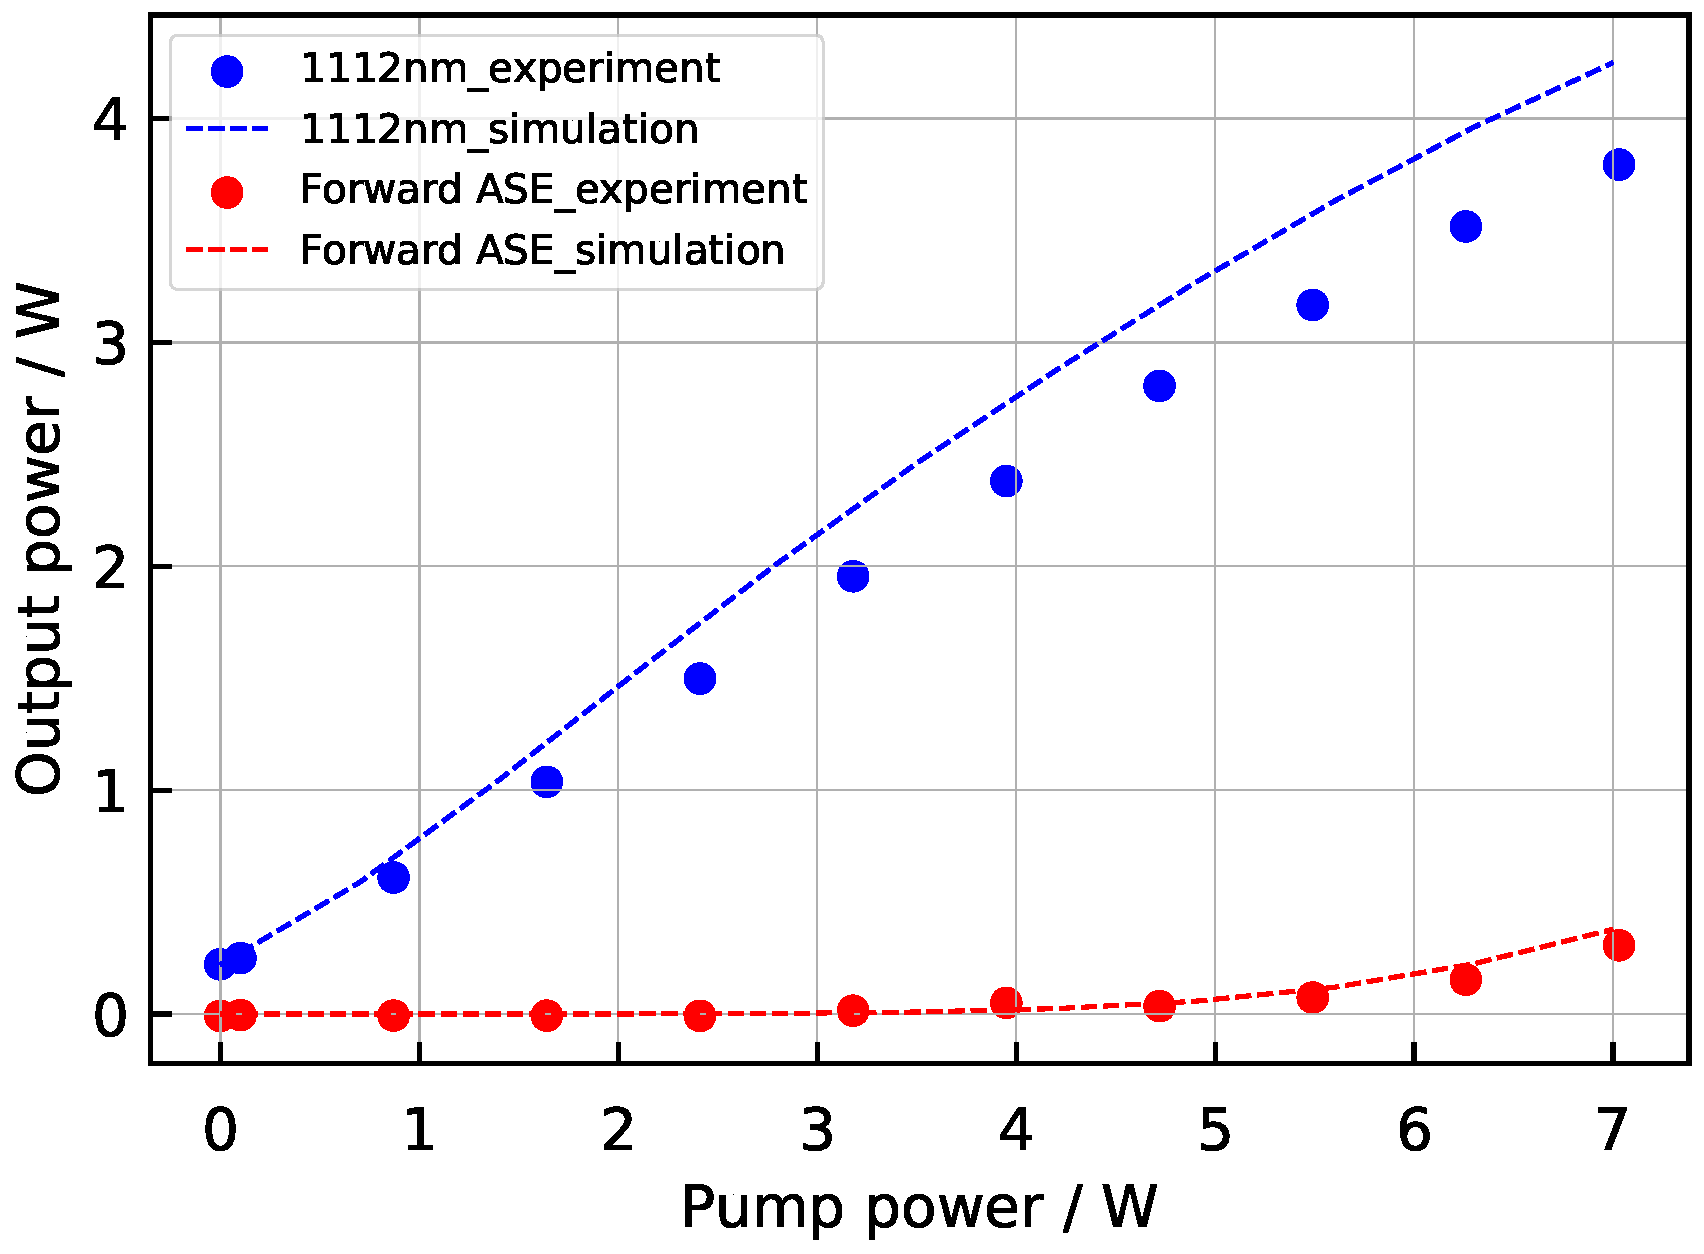
\includegraphics[keepaspectratio, width=0.9\linewidth]{./Figure/1112nmYDFA2ndStageOutput_ComparisonBetweenSimAndExp.pdf}
    \subcaption{}
    \label{fig:ComparisonBetweenSimAndExpOf1112YDFA}
  \end{minipage}
  \begin{minipage}[b]{0.5\linewidth}
    \centering
    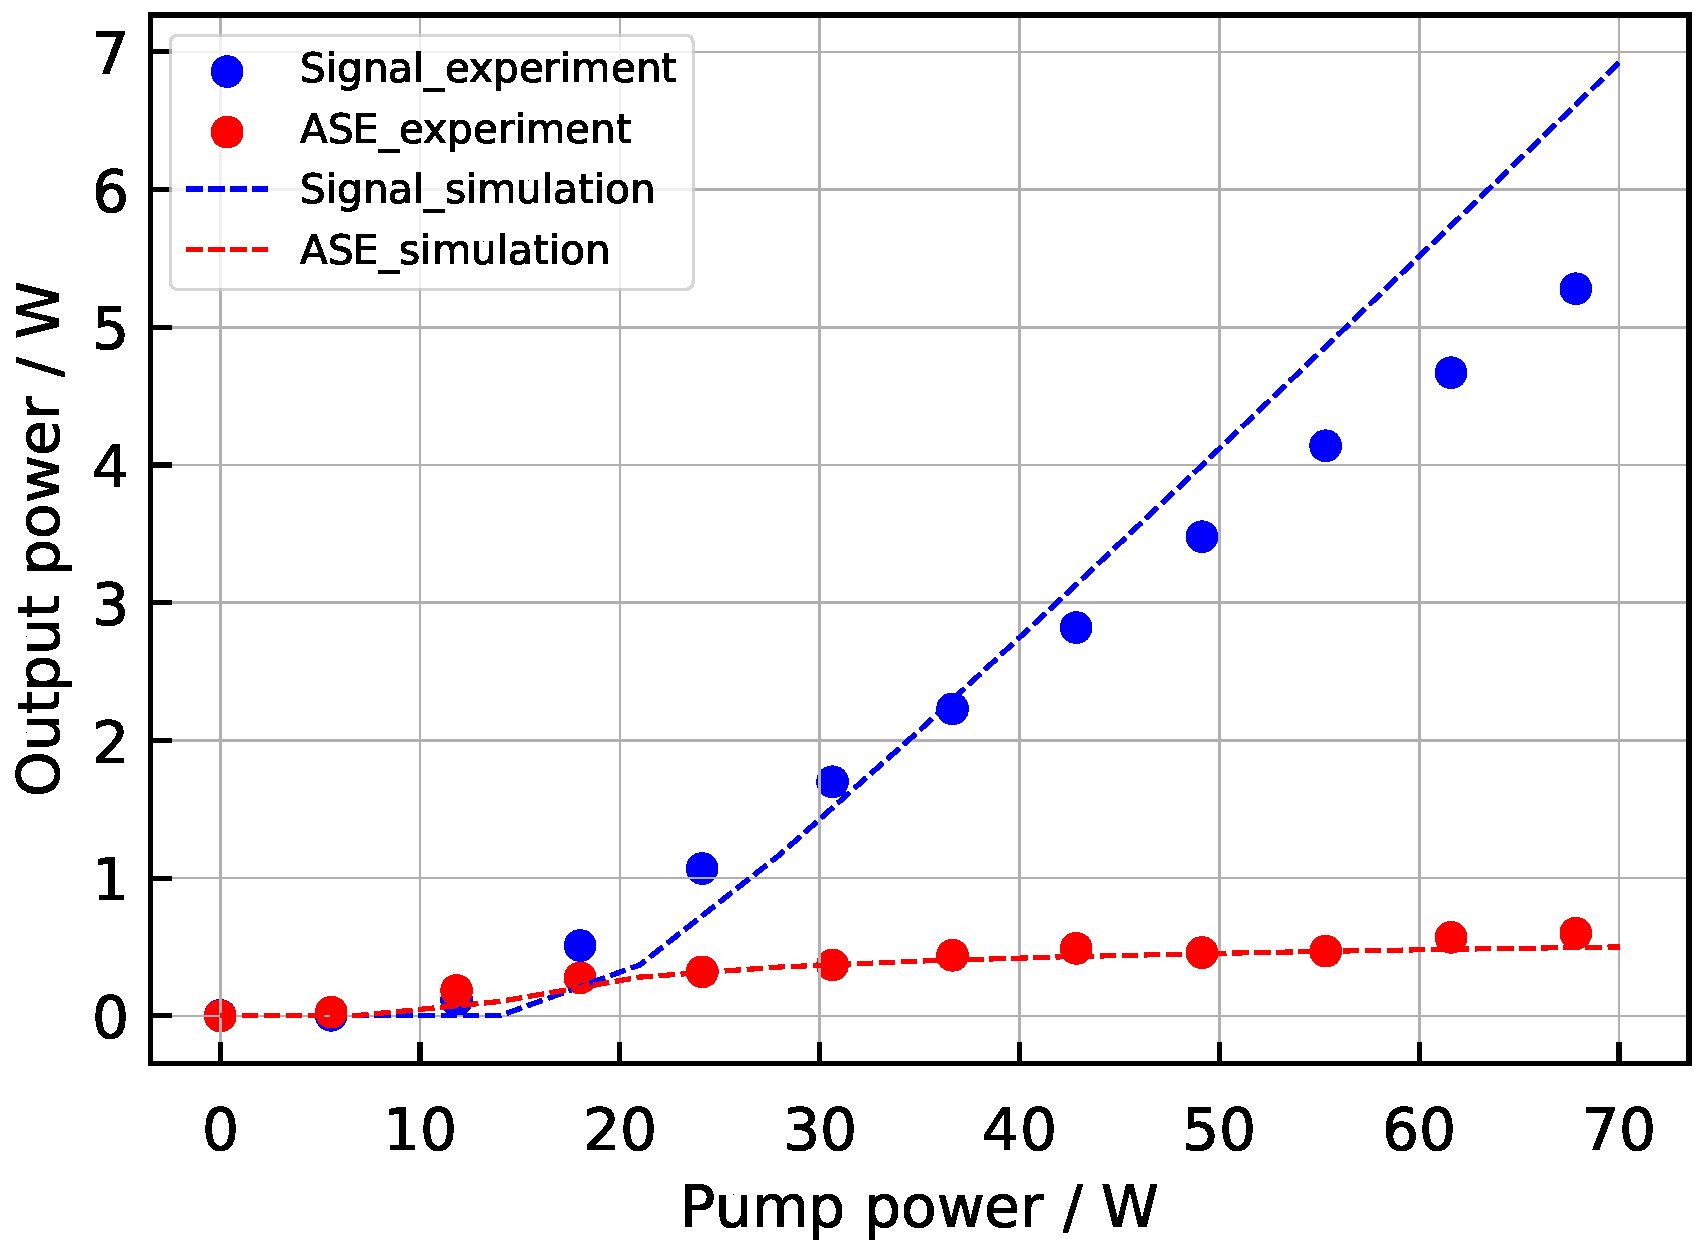
\includegraphics[keepaspectratio, width=0.9\linewidth]{./Figure/976nmYDFAOutput_ComparisonBetweenSimAndExp.pdf}
    \subcaption{}
    \label{fig:ComparisonBetweenSimAndExpOf976YDFA}
  \end{minipage}
  \caption{Comparison between numerical simulation and experimental results of the \SI{976}{\nm} YDFA.}
  \label{fig:ComparisonBetweenSimAndExpOfYDFA}
\end{figure}

We evaluated the experimental results by numerical simulations using \cref{eq:RateEquation,eq:PumpPropagationEquation,eq:SignalPropagationEquation,eq:ASEPropagationEquation} as the model.
Simulation parameters are shown in \cref{tab:SimulationParameters}.
\begin{table}[htbp]
  \caption{Simulation parameters.}
  \label{tab:SimulationParameters}
  \centering
  \begin{tabular}{ccc}
    \hline
    Parameter & 1112YDFA & 976YDFA \\
    \hline \hline
    Yb ion concentration $N$ & $7.3 \times 10^{25}/\si{m^{-3}}$ & $43 \times 10^{25}/\si{m^{-3}}$ \\
    Core diameter & \SI{10}{\um} & \SI{19.8}{\um} \\
    Cladding diameter & \SI{125}{\um} & \SI{128*}{\um} \\
    Core numerical aperture & 0.076 & 0.086 \\
    Pump wavelength $\lambda_{p}$ & \SI{976}{\nm} & \SI{915}{\nm} \\
    Signal wavelength $\lambda_{s}$ & \SI{1112}{\nm} & \SI{976}{\nm} \\
    ASE wavelength $\lambda_{a}$ & \SI{1000-1100}{\nm} & \SI{1000-1100}{\nm} \\
    R1 & $10^{-6}$ & $10^{-6}$ \\
    R2 & $10^{-6}$ & $10^{-6}$ \\
  \end{tabular}
\end{table}
Comparison between the simulation results and experimental results of \SI{1112}{\nm} YDFA shown in Fig.~\ref{fig:ComparisonBetweenSimAndExpOf1112YDFA} indicates good consistency.
The slightly larger experimental result in the forward ASE comparison is probably due to the ASE input at the second stage amplifier caused by residual forward ASE from the first stage amplifier, and re-injection of backward ASE resulting from reflection in upper stream of the \SI{1112}{\nm} system.
Figure \cref{fig:ComparisonBetweenSimAndExpOf976YDFA} shows the result of comparison of \SI{976}{\nm} YDFA.
While the simulated \SI{976}{\nm} output is overestimated relative to its experimental results, the ASE is conversely underestimated.
This may be caused by the fact that the higher-order modes of the ASE were not taken into account in the simulations.
Since the \SI{976}{\nm} seed light is mainly composed of a fundamental mode while the spontaneous emission includes all allowed higher-order modes.
Therefore, the simulation without considering the higher-order modes resulted in large errors in the prediction of the ASE.

\section{Conclusion}
In this paper, we demonstrated the \SI{1112}{\nm} singlemode YDFA and \SI{976}{\nm} few-mode YDFA using only commercial fibers.
By using the Yb-doped fiber with phosphosilicate glass, the power attenuation caused by photodarkening in the \SI{976}{\nm} amplifier which requires a high inversion distribution was suppressed to the same level as that of the \SI{1112}{\nm} amplifier.


\begin{backmatter}

\bmsection{Funding}
JSPS KAKENHI Grant Number JP21K13944

\bmsection{Acknowledgments}


\end{backmatter}

%%%%%%%%%%%%%%%%%%%%%%% References %%%%%%%%%%%%%%%%%%%%%%%%%

%%%%%%%%%% If using BibTeX:
\bibliography{2022YDFA}

%%%%%%%%%% If preparing manually:
% \begin{thebibliography}{1}
% \newcommand{\enquote}[1]{``#1''}

% \bibitem{Zhang:14}
% Y.~Zhang, S.~Qiao, L.~Sun, Q.~W. Shi, W.~Huang, L.~Li, and Z.~Yang,
%   \enquote{Photoinduced active terahertz metamaterials with nanostructured
%   vanadium dioxide film deposited by sol-gel method,}
%   {\protect\JournalTitle{Optics Express}} \textbf{22}, 11070--11078 (2014).

% \bibitem{OSA}
% {Optical Society}, \enquote{{OSA Publishing},}
%   \url{http://www.osapublishing.org}.

% \bibitem{FORSTER2007}
% P.~Forster, V.~Ramaswamy, P.~Artaxo, T.~Bernsten, R.~Betts, D.~Fahey,
%   J.~Haywood, J.~Lean, D.~Lowe, G.~Myhre, J.~Nganga, R.~Prinn, G.~Raga,
%   M.~Schulz, and R.~V. Dorland, \enquote{Changes in atmospheric consituents and
%   in radiative forcing,} in \enquote{Climate Change 2007: The Physical Science
%   Basis. Contribution of Working Group 1 to the Fourth assesment report of
%   Intergovernmental Panel on Climate Change,}  S.~Solomon, D.~Qin, M.~Manning,
%   Z.~Chen, M.~Marquis, K.~B. Averyt, M.~Tignor, and H.~L. Miler, eds.
%   (Cambridge University Press, 2007).

% \end{thebibliography}

\end{document}
